
%% bare_conf.tex
%% V1.4a
%% 2014/09/17
%% by Michael Shell
%% See:
%% http://www.michaelshell.org/
%% for current contact information.
%%
%% This is a skeleton file demonstrating the use of IEEEtran.cls
%% (requires IEEEtran.cls version 1.8a or later) with an IEEE
%% conference paper.
%%
%% Support sites:
%% http://www.michaelshell.org/tex/ieeetran/
%% http://www.ctan.org/tex-archive/macros/latex/contrib/IEEEtran/
%% and
%% http://www.ieee.org/

%%*************************************************************************
%% Legal Notice:
%% This code is offered as-is without any warranty either expressed or
%% implied; without even the implied warranty of MERCHANTABILITY or
%% FITNESS FOR A PARTICULAR PURPOSE! 
%% User assumes all risk.
%% In no event shall IEEE or any contributor to this code be liable for
%% any damages or losses, including, but not limited to, incidental,
%% consequential, or any other damages, resulting from the use or misuse
%% of any information contained here.
%%
%% All comments are the opinions of their respective authors and are not
%% necessarily endorsed by the IEEE.
%%
%% This work is distributed under the LaTeX Project Public License (LPPL)
%% ( http://www.latex-project.org/ ) version 1.3, and may be freely used,
%% distributed and modified. A copy of the LPPL, version 1.3, is included
%% in the base LaTeX documentation of all distributions of LaTeX released
%% 2003/12/01 or later.
%% Retain all contribution notices and credits.
%% ** Modified files should be clearly indicated as such, including  **
%% ** renaming them and changing author support contact information. **
%%
%% File list of work: IEEEtran.cls, IEEEtran_HOWTO.pdf, bare_adv.tex,
%%                    bare_conf.tex, bare_jrnl.tex, bare_conf_compsoc.tex,
%%                    bare_jrnl_compsoc.tex, bare_jrnl_transmag.tex
%%*************************************************************************


% *** Authors should verify (and, if needed, correct) their LaTeX system  ***
% *** with the testflow diagnostic prior to trusting their LaTeX platform ***
% *** with production work. IEEE's font choices and paper sizes can       ***
% *** trigger bugs that do not appear when using other class files.       ***                          ***
% The testflow support page is at:
% http://www.michaelshell.org/tex/testflow/



\documentclass[conference]{Trabalho_3}
\usepackage{graphicx, url, epsfig, subfigure, caption, subcaption}
\usepackage{amsmath, amscd, amsthm, amsxtra}
\usepackage[T1]{fontenc}
\usepackage[brazil]{babel}   
\usepackage[latin1]{inputenc}
\usepackage{listings}
\usepackage{color}
\usepackage{verbatim}

% Some Computer Society conferences also require the compsoc mode option,
% but others use the standard conference format.
%
% If IEEEtran.cls has not been installed into the LaTeX system files,
% manually specify the path to it like:
% \documentclass[conference]{../sty/IEEEtran}





% Some very useful LaTeX packages include:2
% (uncomment the ones you want to load)


% *** MISC UTILITY PACKAGES ***
%
%\usepackage{ifpdf}
% Heiko Oberdiek's ifpdf.sty is very useful if you need conditional
% compilation based on whether the output is pdf or dvi.
% usage:
% \ifpdf
%   % pdf code
% \else
%   % dvi code
% \fi
% The latest version of ifpdf.sty can be obtained from:
% http://www.ctan.org/tex-archive/macros/latex/contrib/oberdiek/
% Also, note that IEEEtran.cls V1.7 and later provides a builtin
% \ifCLASSINFOpdf conditional that works the same way.
% When switching from latex to pdflatex and vice-versa, the compiler may
% have to be run twice to clear warning/error messages.






% *** CITATION PACKAGES ***
%
%\usepackage{cite}
% cite.sty was written by Donald Arseneau
% V1.6 and later of IEEEtran pre-defines the format of the cite.sty package
% \cite{} output to follow that of IEEE. Loading the cite package will
% result in citation numbers being automatically sorted and properly
% "compressed/ranged". e.g., [1], [9], [2], [7], [5], [6] without using
% cite.sty will become [1], [2], [5]--[7], [9] using cite.sty. cite.sty's
% \cite will automatically add leading space, if needed. Use cite.sty's
% noadjust option (cite.sty V3.8 and later) if you want to turn this off
% such as if a citation ever needs to be enclosed in parenthesis.
% cite.sty is already installed on most LaTeX systems. Be sure and use
% version 5.0 (2009-03-20) and later if using hyperref.sty.
% The latest version can be obtained at:
% http://www.ctan.org/tex-archive/macros/latex/contrib/cite/
% The documentation is contained in the cite.sty file itself.






% *** GRAPHICS RELATED PACKAGES ***
%
\ifCLASSINFOpdf
  % \usepackage[pdftex]{graphicx}
  % declare the path(s) where your graphic files are
  % \graphicspath{{../pdf/}{../jpeg/}}
  % and their extensions so you won't have to specify these with
  % every instance of \includegraphics
  % \DeclareGraphicsExtensions{.pdf,.jpeg,.png}
\else
  % or other class option (dvipsone, dvipdf, if not using dvips). graphicx
  % will default to the driver specified in the system graphics.cfg if no
  % driver is specified.
  % \usepackage[dvips]{graphicx}
  % declare the path(s) where your graphic files are
  % \graphicspath{{../eps/}}
  % and their extensions so you won't have to specify these with
  % every instance of \includegraphics
  % \DeclareGraphicsExtensions{.eps}
\fi
% graphicx was written by David Carlisle and Sebastian Rahtz. It is
% required if you want graphics, photos, etc. graphicx.sty is already
% installed on most LaTeX systems. The latest version and documentation
% can be obtained at: 
% http://www.ctan.org/tex-archive/macros/latex/required/graphics/
% Another good source of documentation is "Using Imported Graphics in
% LaTeX2e" by Keith Reckdahl which can be found at:
% http://www.ctan.org/tex-archive/info/epslatex/
%
% latex, and pdflatex in dvi mode, support graphics in encapsulated
% postscript (.eps) format. pdflatex in pdf mode supports graphics
% in .pdf, .jpeg, .png and .mps (metapost) formats. Users should ensure
% that all non-photo figures use a vector format (.eps, .pdf, .mps) and
% not a bitmapped formats (.jpeg, .png). IEEE frowns on bitmapped formats
% which can result in "jaggedy"/blurry rendering of lines and letters as
% well as large increases in file sizes.
%
% You can find documentation about the pdfTeX application at:
% http://www.tug.org/applications/pdftex





% *** MATH PACKAGES ***
%
%\usepackage[cmex10]{amsmath}
% A popular package from the American Mathematical Society that provides
% many useful and powerful commands for dealing with mathematics. If using
% it, be sure to load this package with the cmex10 option to ensure that
% only type 1 fonts will utilized at all point sizes. Without this option,
% it is possible that some math symbols, particularly those within
% footnotes, will be rendered in bitmap form which will result in a
% document that can not be IEEE Xplore compliant!
%
% Also, note that the amsmath package sets \interdisplaylinepenalty to 10000
% thus preventing page breaks from occurring within multiline equations. Use:
%\interdisplaylinepenalty=2500
% after loading amsmath to restore such page breaks as IEEEtran.cls normally
% does. amsmath.sty is already installed on most LaTeX systems. The latest
% version and documentation can be obtained at:
% http://www.ctan.org/tex-archive/macros/latex/required/amslatex/math/





% *** SPECIALIZED LIST PACKAGES ***
%
%\usepackage{algorithmic}
% algorithmic.sty was written by Peter Williams and Rogerio Brito.
% This package provides an algorithmic environment fo describing algorithms.
% You can use the algorithmic environment in-text or within a figure
% environment to provide for a floating algorithm. Do NOT use the algorithm
% floating environment provided by algorithm.sty (by the same authors) or
% algorithm2e.sty (by Christophe Fiorio) as IEEE does not use dedicated
% algorithm float types and packages that provide these will not provide
% correct IEEE style captions. The latest version and documentation of
% algorithmic.sty can be obtained at:
% http://www.ctan.org/tex-archive/macros/latex/contrib/algorithms/
% There is also a support site at:
% http://algorithms.berlios.de/index.html
% Also of interest may be the (relatively newer and more customizable)
% algorithmicx.sty package by Szasz Janos:
% http://www.ctan.org/tex-archive/macros/latex/contrib/algorithmicx/




% *** ALIGNMENT PACKAGES ***
%
%\usepackage{array}
% Frank Mittelbach's and David Carlisle's array.sty patches and improves
% the standard LaTeX2e array and tabular environments to provide better
% appearance and additional user controls. As the default LaTeX2e table
% generation code is lacking to the point of almost being broken with
% respect to the quality of the end results, all users are strongly
% advised to use an enhanced (at the very least that provided by array.sty)
% set of table tools. array.sty is already installed on most systems. The
% latest version and documentation can be obtained at:
% http://www.ctan.org/tex-archive/macros/latex/required/tools/


% IEEEtran contains the IEEEeqnarray family of commands that can be used to
% generate multiline equations as well as matrices, tables, etc., of high
% quality.




% *** SUBFIGURE PACKAGES ***
%\ifCLASSOPTIONcompsoc
%  \usepackage[caption=false,font=normalsize,labelfont=sf,textfont=sf]{subfig}
%\else
%  \usepackage[caption=false,font=footnotesize]{subfig}
%\fi
% subfig.sty, written by Steven Douglas Cochran, is the modern replacement
% for subfigure.sty, the latter of which is no longer maintained and is
% incompatible with some LaTeX packages including fixltx2e. However,
% subfig.sty requires and automatically loads Axel Sommerfeldt's caption.sty
% which will override IEEEtran.cls' handling of captions and this will result
% in non-IEEE style figure/table captions. To prevent this problem, be sure
% and invoke subfig.sty's "caption=false" package option (available since
% subfig.sty version 1.3, 2005/06/28) as this is will preserve IEEEtran.cls
% handling of captions.
% Note that the Computer Society format requires a larger sans serif font
% than the serif footnote size font used in traditional IEEE formatting
% and thus the need to invoke different subfig.sty package options depending
% on whether compsoc mode has been enabled.
%
% The latest version and documentation of subfig.sty can be obtained at:
% http://www.ctan.org/tex-archive/macros/latex/contrib/subfig/




% *** FLOAT PACKAGES ***
%
%\usepackage{fixltx2e}
% fixltx2e, the successor to the earlier fix2col.sty, was written by
% Frank Mittelbach and David Carlisle. This package corrects a few problems
% in the LaTeX2e kernel, the most notable of which is that in current
% LaTeX2e releases, the ordering of single and double column floats is not
% guaranteed to be preserved. Thus, an unpatched LaTeX2e can allow a
% single column figure to be placed prior to an earlier double column
% figure. The latest version and documentation can be found at:
% http://www.ctan.org/tex-archive/macros/latex/base/


%\usepackage{stfloats}
% stfloats.sty was written by Sigitas Tolusis. This package gives LaTeX2e
% the ability to do double column floats at the bottom of the page as well
% as the top. (e.g., "\begin{figure*}[!b]" is not normally possible in
% LaTeX2e). It also provides a command:
%\fnbelowfloat
% to enable the placement of footnotes below bottom floats (the standard
% LaTeX2e kernel puts them above bottom floats). This is an invasive package
% which rewrites many portions of the LaTeX2e float routines. It may not work
% with other packages that modify the LaTeX2e float routines. The latest
% version and documentation can be obtained at:
% http://www.ctan.org/tex-archive/macros/latex/contrib/sttools/
% Do not use the stfloats baselinefloat ability as IEEE does not allow
% \baselineskip to stretch. Authors submitting work to the IEEE should note
% that IEEE rarely uses double column equations and that authors should try
% to avoid such use. Do not be tempted to use the cuted.sty or midfloat.sty
% packages (also by Sigitas Tolusis) as IEEE does not format its papers in
% such ways.
% Do not attempt to use stfloats with fixltx2e as they are incompatible.
% Instead, use Morten Hogholm'a dblfloatfix which combines the features
% of both fixltx2e and stfloats:
%
% \usepackage{dblfloatfix}
% The latest version can be found at:
% http://www.ctan.org/tex-archive/macros/latex/contrib/dblfloatfix/




% *** PDF, URL AND HYPERLINK PACKAGES ***
%
%\usepackage{url}
% url.sty was written by Donald Arseneau. It provides better support for
% handling and breaking URLs. url.sty is already installed on most LaTeX
% systems. The latest version and documentation can be obtained at:
% http://www.ctan.org/tex-archive/macros/latex/contrib/url/
% Basically, \url{my_url_here}.




% *** Do not adjust lengths that control margins, column widths, etc. ***
% *** Do not use packages that alter fonts (such as pslatex).         ***
% There should be no need to do such things with IEEEtran.cls V1.6 and later.
% (Unless specifically asked to do so by the journal or conference you plan
% to submit to, of course. )


% correct bad hyphenation here
\hyphenation{op-tical net-works semi-conduc-tor}


\begin{document}
%
% paper title
% Titles are generally capitalized except for words such as a, an, and, as,
% at, but, by, for, in, nor, of, on, or, the, to and up, which are usually
% not capitalized unless they are the first or last word of the title.
% Linebreaks \\ can be used within to get better formatting as desired.
% Do not put math or special symbols in the title.
\title{Pr\'e-processamento e Quantiza\c{c}\~ao em Codifica\c{c}\~ao com Perdas}


% author names and affiliations
% use a multiple column layout for up to three different
% affiliations
\author{\IEEEauthorblockN{Rodrigo Ferreira Guimar\~aes}
\IEEEauthorblockA{Departamento de Ci\^encia de Computa\c{c}\~ao e Faculdade de Tecnologia\\
Universidade de Bras\'ilia, Bras\'ilia\\
Email: rodrigofegui@aluno.unb.br\\
Matr\'icula: 14/0170740}
}

% conference papers do not typically use \thanks and this command
% is locked out in conference mode. If really needed, such as for
% the acknowledgment of grants, issue a \IEEEoverridecommandlockouts
% after \documentclass

% for over three affiliations, or if they all won't fit within the width
% of the page, use this alternative format:
% 
%\author{\IEEEauthorblockN{Michael Shell\IEEEauthorrefmark{1},
%Homer Simpson\IEEEauthorrefmark{2},
%James Kirk\IEEEauthorrefmark{3}, 
%Montgomery Scott\IEEEauthorrefmark{3} and
%Eldon Tyrell\IEEEauthorrefmark{4}}
%\IEEEauthorblockA{\IEEEauthorrefmark{1}School of Electrical and Computer Engineering\\
%Georgia Institute of Technology,
%Atlanta, Georgia 30332--0250\\ Email: see http://www.michaelshell.org/contact.html}
%\IEEEauthorblockA{\IEEEauthorrefmark{2}Twentieth Century Fox, Springfield, USA\\
%Email: homer@thesimpsons.com}
%\IEEEauthorblockA{\IEEEauthorrefmark{3}Starfleet Academy, San Francisco, California 96678-2391\\
%Telephone: (800) 555--1212, Fax: (888) 555--1212}
%\IEEEauthorblockA{\IEEEauthorrefmark{4}Tyrell Inc., 123 Replicant Street, Los Angeles, California 90210--4321}}




% use for special paper notices
%\IEEEspecialpapernotice{(Invited Paper)}




% make the title area
\maketitle

% As a general rule, do not put math, special symbols or citations
% in the abstract
%\begin{abstract}
%O resumo vem aqui.
%\end{abstract}

% no keywords




% For peer review papers, you can put extra information on the cover
% page as needed:
% \ifCLASSOPTIONpeerreview
% \begin{center} \bfseries EDICS Category: 3-BBND \end{center}
% \fi
%
% For peerreview papers, this IEEEtran command inserts a page break and
% creates the second title. It will be ignored for other modes.
\IEEEpeerreviewmaketitle


%%%%%%%%%%%%%%%%%%%%%%%%%%%%%%%%%%%%%%%%%%%%%%%%%%%%%%%%%%%%%%%%%%%%%%%%%%%%%
\section{Introdu\c{c}\~ao}
  \label{intro}
%%%%%%%%%%%%%%%%%%%%%%%%%%%%%%%%%%%%%%%%%%%%%%%%%%%%%%%%%%%%%%%%%%%%%%%%%%%%%
Este trabalho visa fixar os conceitos relativos a realce no dom\'inio espacial, filtragem no dom\'inio da frequ\^encia e de morfologia matem\'atica. Para atingir tal objetivo foram consideradas tr\^es imagens-base e dois problemas:~\textbf{a)} aplicar a DCT em duas dimens\~oes, seguida pela quantiza\c{c}\~ao e pela DCT inversa;~\textbf{b)} similar ao anterior, com a difer\^en\c{c}a de que deve ser realizada o DPCM antes dos passos j\'a descritos. Para ambos os problemas foram realizadas an\'alises sobre a vari\^ancia dos blocos requantizados e sobre a PSNR entre as imagens.
 
\hfill 30 de novembro, 2015


% An example of a floating figure using the graphicx package.
% Note that \label must occur AFTER (or within) \caption.
% For figures, \caption should occur after the \includegraphics.
% Note that IEEEtran v1.7 and later has special internal code that
% is designed to preserve the operation of \label within \caption
% even when the captionsoff option is in effect. However, because
% of issues like this, it may be the safest practice to put all your
% \label just after \caption rather than within \caption{}.
%
% Reminder: the "draftcls" or "draftclsnofoot", not "draft", class
% option should be used if it is desired that the figures are to be
% displayed while in draft mode.
%
%\begin{figure}[!t]
%\centering
%\includegraphics[width=2.5in]{myfigure}
% where an .eps filename suffix will be assumed under latex, 
% and a .pdf suffix will be assumed for pdflatex; or what has been declared
% via \DeclareGraphicsExtensions.
%\caption{Simulation results for the network.}
%\label{fig_sim}
%\end{figure}

% Note that IEEE typically puts floats only at the top, even when this
% results in a large percentage of a column being occupied by floats.


% An example of a double column floating figure using two subfigures.
% (The subfig.sty package must be loaded for this to work.)
% The subfigure \label commands are set within each subfloat command,
% and the \label for the overall figure must come after \caption.
% \hfil is used as a separator to get equal spacing.
% Watch out that the combined width of all the subfigures on a 
% line do not exceed the text width or a line break will occur.
%
%\begin{figure*}[!t]
%\centering
%\subfloat[Case I]{\includegraphics[width=2.5in]{box}%
%\label{fig_first_case}}
%\hfil
%\subfloat[Case II]{\includegraphics[width=2.5in]{box}%
%\label{fig_second_case}}
%\caption{Simulation results for the network.}
%\label{fig_sim}
%\end{figure*}
%
% Note that often IEEE papers with subfigures do not employ subfigure
% captions (using the optional argument to \subfloat[]), but instead will
% reference/describe all of them (a), (b), etc., within the main caption.
% Be aware that for subfig.sty to generate the (a), (b), etc., subfigure
% labels, the optional argument to \subfloat must be present. If a
% subcaption is not desired, just leave its contents blank,
% e.g., \subfloat[].


% An example of a floating table. Note that, for IEEE style tables, the
% \caption command should come BEFORE the table and, given that table
% captions serve much like titles, are usually capitalized except for words
% such as a, an, and, as, at, but, by, for, in, nor, of, on, or, the, to
% and up, which are usually not capitalized unless they are the first or
% last word of the caption. Table text will default to \footnotesize as
% IEEE normally uses this smaller font for tables.
% The \label must come after \caption as always.
%
%\begin{table}[!t]
%% increase table row spacing, adjust to taste
%\renewcommand{\arraystretch}{1.3}
% if using array.sty, it might be a good idea to tweak the value of
% \extrarowheight as needed to properly center the text within the cells
%\caption{An Example of a Table}
%\label{table_example}
%\centering
%% Some packages, such as MDW tools, offer better commands for making tables
%% than the plain LaTeX2e tabular which is used here.
%\begin{tabular}{|c||c|}
%\hline
%One & Two\\
%\hline
%Three & Four\\
%\hline
%\end{tabular}
%\end{table}


% Note that the IEEE does not put floats in the very first column
% - or typically anywhere on the first page for that matter. Also,
% in-text middle ("here") positioning is typically not used, but it
% is allowed and encouraged for Computer Society conferences (but
% not Computer Society journals). Most IEEE journals/conferences use
% top floats exclusively. 
% Note that, LaTeX2e, unlike IEEE journals/conferences, places
% footnotes above bottom floats. This can be corrected via the
% \fnbelowfloat command of the stfloats package.

%%%%%%%%%%%%%%%%%%%%%%%%%%%%%%%%%%%%%%%%%%%%%%%%%%%%%%%%%%%%%%%%%%%%%%%%%%%%%
\section{Embasamento Te\'orico}
  \label{teorico}
%%%%%%%%%%%%%%%%%%%%%%%%%%%%%%%%%%%%%%%%%%%%%%%%%%%%%%%%%%%%%%%%%%%%%%%%%%%%%
Para que haja um correto entendimento sobre o desenvolvimento deste projeto \'e importante abordar alguns aspectos relevantes, como as defini\c{c}\~oes: de uma imagem; codifica\c{c}\~ao de imagens; da DCT e sua inversa; do DPCM; da PSNR, dentre outros assuntos.

%%%%%%%%%%%%%%%%%%%%%%%%%%%%%%%%%%%%%%%
\subsection{Imagem e~\textit{Pixels}}
  \label{imagens}
%%%%%%%%%%%%%%%%%%%%%%%%%%%%%%%%%%%%%%%
Uma imagem pode ser definida como uma fun\c{c}\~ao bidimensional do tipo $f(x,y)$, onde $x$ e $y$ s\~ao as coordenadas espaciais e a amplitude de $f$ em qualquer ponto de coordenadas $(x,y)$ \'e denominado de intensidade da imagem naquele ponto. Quando $x$, $y$ e $f$ s\~ao valores~\textit{finitos} e~\textit{discretos}, a imagem \'e denominada imagem digital, tendo esta signific\^ancia aos computadores digitais. Um dado elemento com coordenadas $(x,y)$ e intensidade $f$ \'e denominado de~\textit{pixel}~(picture element ou, em portugu\^es, elemento de imagem), dessa forma, entende-se que uma imagem \'e constituida por um ou mais~\textit{pixels}.

Para a manipula\c{c}\~ao dos~\textit{pixels} \'e necess\'ario saber as rela\c{c}\~oes b\'asicas entre eles, como, por exemplo, a vizinhan\c{c}a. Os conceito a serem apresentados consideram uma imagem em n\'ivel de cinza.

Cada~\textit{pixel} $p$ pode possui tr\^es tipos de vizinhan\c{c}a, semelhantes a Rosa-dos-Ventos da Figura~\ref{fig:rosadosventos}:~\textit{vizinhan\c{c}a de 4},~\textit{vizinhan\c{c}a diagonal} e~\textit{vizinhan\c{c}a de 8}; onde para o primeiro, denonato por $N_4$(p), s\~ao considerados os quatro vizinhos horizontais e verticais, seguindo as orienta\c{c}\~oes~\textit{N-S-L-O} da Rosa-dos-Ventos; para o segundo, denonato por $N_D$(p), s\~ao considerados os vizinhos das diagonais, seguindo as orienta\c{c}\~oes~\textit{NE-SE-SO-NO}; enquanto que o terceiro tipo, denonato por $N_8$(p), \'e a jun\c{c}\~ao dos dois anteriores.

\begin{figure}[!t]
  \centering
  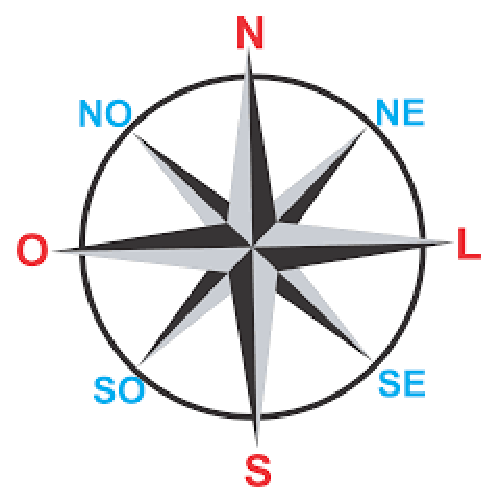
\includegraphics[width = 3.5 cm]{rosadosventos}
  \caption{Sinaliza\c{c}\~ao dos sentido cardeias da Rosa-dos-Ventos. Fonte~\cite{rosadosventos}.}
  \label{fig:rosadosventos}
\end{figure}

%%%%%%%%%%%%%%%%%%%%%%%%%%%%%%%%%%%%%%%
\subsection{Codifica\c{c}\~ao de Imagens}
  \label{cod}
%%%%%%%%%%%%%%%%%%%%%%%%%%%%%%%%%%%%%%%
Ao considerar que sinais possuem dados reduntantes e que imagens s\~ao sinais, digitais, ent\~ao tem-se que as imagens possuem dados reduntantes. O ramo do processamento de imagens que lida com estes dados reduntantes \'e a codifica\c{c}a\~ao, pois objetiva diminuir a quantidade de dados necess\'arios para a reconstru\c{c}\~ao da imagem sem a perda de qualidade aliada a um fator de codifica\c{c}a\~ao, havendo duas formas de se trabalhar: com ou sem perdas (\textit{lossy} ou \textit{lossless}, respectivamente). Para este projeto \'e aplicada uma parte da codifica\c{c}a\~ao com perdas.

A principal caracter\'istica da codifica\c{c}a\~ao com perdas \'e o fato de que a imagem reconstru\'ida n\~ao \'e id\^entica \`a original, mas possui somente as informa\c{c}\~oes \'uteis aos olhos humanos.

Os codificadores com perdas possuem um esquema padr\~ao quanto aos passos a serem seguidos, de forma geral, sendo eles:~\textit{\textbf{a)}} pr\'e-pocessamento, consiste na remo\c{c}\~ao de redund\^ancias e transformadas para o dom\'inio da frequ\^encia, por exemplo, sendo um processo revers\'ivel;~\textit{\textbf{b)}} quantizador, transforma o alfabeto de s\'imbolos para um outro de conjunto mais limitado, sendo um processo irrevers\'ivel;~\textit{\textbf{c)}} codificador entr\'opico, consiste em codificar os s\'imbolos numa sequ\^encia de~\textit{bits} que possa ser enviada ao decodificador.

%%%%%%%%%%%%%%%%%%%%%%%%%%%%%%%%%%%%%%%
\subsection{DCT e sua Inversa}
  \label{dct}
%%%%%%%%%%%%%%%%%%%%%%%%%%%%%%%%%%%%%%%
A DCT (\textit{Discrete Cosine Transform} ou, em portugu\^es, Transformada Discreta de Cosseno) \'e uma ferramenta important para o processamento de imagens, proporciona alta efici\^encia no c\'alculo e excelente compress\c{c}ao.

\'E esperado que os dados reais da entrada tenham uma transi\c{c}\~ao, quase, cont\'inua para a sua vizinha. Dessa forma, a DCT funciona na base que os primeiros elementos tenham vizinhos de pouca varia\c{c}\~ao e os \'ultimos tenham grande vari\^ancia, ou seja, os primeiros est\~ao nas baixas frequ\^encias e os \'ultimos nas altas frequ\^encias. Assim, ao realizar uma combina\c{c}\~ao linear da base com os dados de entradas, \'e esperado que os coeficientes de maior magnitude sejam os primeiro, enquanto que os \'ultimos coeficientes sejam praticamente nulos, podendo ser desprez\'iveis.

Ao ser aplicado em imagens, \'e utilizada a DCT bidimensional, sendo calculada a apartir da equa\c{c}\~ao da Figura~\ref{fig:DCT}.

\begin{figure}
  \centering
  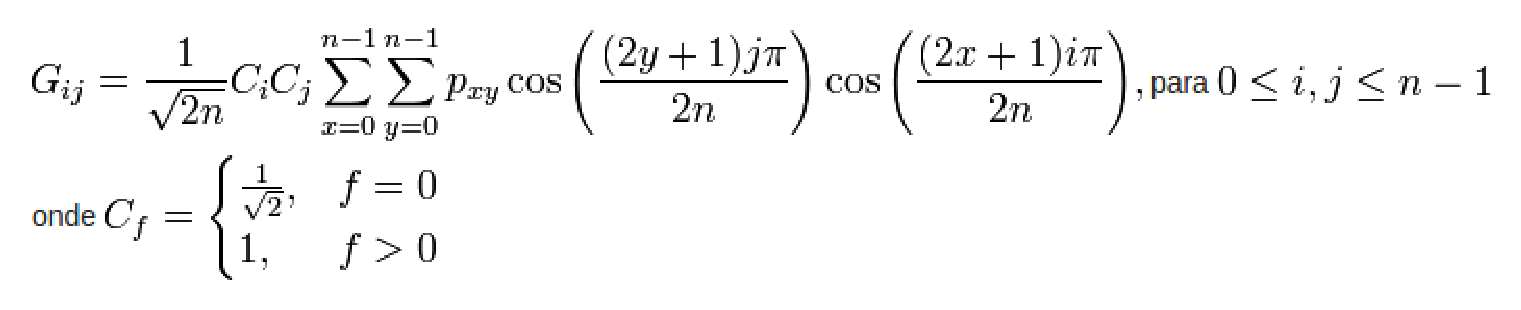
\includegraphics[width = 9 cm]{DCT}
  \caption{Equa\c{c}\~ao da DCT bidimensional.}
  \label{fig:DCT}
\end{figure}

Como a DCT leva do dom\'inio espacial ao da frequ\^encia \'e preciso ter uma outra ferramenta que fa\c{c}a o ``caminho'' da volta, por isso que existe a DCT inversa.

Vale ressaltar que a DCT, aplicada a este projeto, manipula blocos de ${8 \times 8}$~\textit{pixels}.

%%%%%%%%%%%%%%%%%%%%%%%%%%%%%%%%%%%%%%%
\subsection{DPCM}
  \label{dpcm}
%%%%%%%%%%%%%%%%%%%%%%%%%%%%%%%%%%%%%%%
Sabendo que uma imagem \'e um sinal anal\'ogico amostrado, o DPCM  (\textit{Differential Pulse-Code Modulation} ou, em portugu\^es, Diferencial de Modula\c{c}\~ao por Codifica\c{c}\~ao de Pulso) realiza a quantiza\c{c}\~ao de um sinal de erro, comumente denominado erro de predi\c{c}\~ao. Tal erro \'e obtido pela diferen\c{c}a entre o sinal amostrado e o sinal estimado pelo preditor linear.

Dessa forma, objetiva-se minimizar o erro m\'edio quadr\'atico de predi\c{c}\~ao, uma vez que o erro \'e assumido desprez\'ivel e que o valor predito \'e uma combina\c{c}\~ao linear de $m$~\textit{pixels} anteriores.

%%%%%%%%%%%%%%%%%%%%%%%%%%%%%%%%%%%%%%%
\subsection{PSNR}
  \label{psnr}
%%%%%%%%%%%%%%%%%%%%%%%%%%%%%%%%%%%%%%%
A PSNR (\textit{Peak Signal-to-Noise Ratio} ou, em portugu\^es, Rela\c{c}\~ao Sinal-Ru\'ido de Pico), aplica a imagens, representa a medida quantitativa da qualidade de reconstru\c{c}\~ao, focada a codifica\c{c}a\~ao de imagens. Para determinar seu valor, que \'e expresso em escala logar\'itmica, cuja unidade \'e o decibel, \'e importante determinar o~\textit{erro quadr\'atico m\'edio} ($MSE$), seguinte esta equa\c{c}\~ao:
$$MSE = {{1} \over {MN}} \sum\limits_{i = 1}^{M - 1}\sum\limits_{j = 1}^{N - 1}{\mid I(i,j) - K(i,j) \mid ^ 2},$$ onde $I$ e $K$ s\~ao as imagens. Com o $MSE$ definido \'e poss\'ivel, ent\~ao, definir a $PSNR$ em si, sendo ela determinada atrav\'es desta equa\c{c}\~ao ou qualquer manipula\c{c}\~ao alg\'ebrica da mesma:
$$PSNR = 10 \cdot log_{10}\left({{MAX_I}^2 \over {MSE}}\right),$$ onde $MAX_I$ \'e o valor m\'aximo poss\'ivel para as imagens, que neste projeto corresponde a $255$.

%%%%%%%%%%%%%%%%%%%%%%%%%%%%%%%%%%%%%%%
\subsection{Vari\^ancia}
  \label{var}
%%%%%%%%%%%%%%%%%%%%%%%%%%%%%%%%%%%%%%%
A vari\^ancia ($Var(x)$) a vari\'avel aleat\'oria \'e a medida da sua dispers\~ao estat\'istica ao indicar a difer\^encia dos valores reais em relac\c{c}\~ao ao valor esperado. Sendo definida pela equa\c{c}\~ao:
$$Var(x) =  {{1} \over {N - 1}} \sum\limits_{i = 1}^{N}{\mid{X_i - E(x)}\mid^2},$$ onde $E(x)$ \'e o valor esperado, tamb\'em denominado de~\textit{esperan\c{c}a}, enquanto que $X_i$ \'e o valor real das amostras.

%%%%%%%%%%%%%%%%%%%%%%%%%%%%%%%%%%%%%%%%%%%%%%%%%%%%%%%%%%%%%%%%%%%%%%%%%%%%%
\section{Metodologia}
  \label{metodo}
%%%%%%%%%%%%%%%%%%%%%%%%%%%%%%%%%%%%%%%%%%%%%%%%%%%%%%%%%%%%%%%%%%%%%%%%%%%%%
Com as defini\c{c}\~oes feitas \'e poss\'ivel prosseguir para o desenvolvimento do projeto. Dessa forma, esta se\c{c}\~ao visa apresentar os passos seguidos para a realiza\c{c}\~ao das atividades, desenvolvidas em ~\textbf{\textit{MatLab}}~\cite{matlab}. Como o projeto \'e constitu\'ido por dois problemas, estes ser\~ao abordados separadamente.

%%%%%%%%%%%%%%%%%%%%%%%%%%%%%%%%%%%%%%%
\subsection{Simples Codifica\c{c}\~ao com Perdas}
  \label{codilossy_metodo}
%%%%%%%%%%%%%%%%%%%%%%%%%%%%%%%%%%%%%%%
Como informado na Se\c{c}\~ao~\ref{intro}, este problema consiste em aplica a DCT numa imagem, seguida pela quantiza\c{c}\~ao em n\'ives pr\'e-estabelecidos e pela DCT inversa. Os n\'ives de quantiza\c{c}\~ao considerados foram: $1$, $10$, $20$, $50$ e $100$.

Primeiramente foi realizado um~\textit{padding} nas imagens, pois, como informado na Se\c{c}\~ao~\ref{dct}, a DCT manipula blocos de ${8 \times 8}$~\textit{pixels}, logo \'e preciso ajustar as imagens a esta propor\c{c}\~ao e para este projeto foi~\textit{padding} de zeros.

Em seguida a imagem foi manipulada de bloco em bloco, sendo aplicada esta sequ\^encia de passos:~\textbf{a)} DCT sobre o bloco, seguida pela divis\~ao pelo passo de quantiza\c{c}\~ao e pelo arredondamento para $-\infty$ (fun\c{c}\~ao \textit{floor});~\textbf{b)} foi calculada a m\'edia das vari\^ancias das colunas do bloco transformado;~\textbf{c)} o bloco foi decodificado atrav\'es da DCT inversa, seguido pela multiplica\c{c}\~ao pelo passo de quantiza\c{c}\~ao.

Ao finalizar as manipula\c{c}\~oes nos blocos o~\textit{padding} foi removido, a vari\^ancia m\'edia para toda a imagem foi determinada, al\'em da determina\c{c}\~ao da PSNR da imagem reconstru\'ida com a imagem original.

%%%%%%%%%%%%%%%%%%%%%%%%%%%%%%%%%%%%%%%
\subsection{DPCM antes da Codifica\c{c}\~ao}
  \label{dpcmlossy_metodo}
%%%%%%%%%%%%%%%%%%%%%%%%%%%%%%%%%%%%%%%
Tem um procedimento totalmente an\'alogo ao descrito na Se\c{c}\~ao~\ref{codilossy_metodo}, o diferencial est\'a na inser\c{c}\~ao do DCPM.

Considerando que o bloco corrente est\'a na posi\c{c}\~ao $(x, y)$ e que a predi\c{c}ao realizada considerao o bloco na posi\c{c}\~ao $(x, y - 1)$, ent\~ao para o primeiro bloco a predi\c{c}\~ao \'e envi\'avel. Mas para os seguintes, a predi\c{c}\~ao sobre cada~\textit{pixel} \'e realizada sobre o~\textit{pixel} corresponte do bloco base da predi\c{c}\~ao.

A predi\c{c}\~ao \'e a difer\^en\c{c}a do~\textit{pixel} corrente com o~\textit{pixel} correspondente no bloco j\'a decodificado. Ap\'os a predi\c{c}\~ao ocorre o procedimento j\'a descrito e h\'a o la\c{c}o das a\c{c}\~oes at\'e que o bloco corrente seja o \'ultimo bloco da linha de blocos.


%%%%%%%%%%%%%%%%%%%%%%%%%%%%%%%%%%%%%%%%%%%%%%%%%%%%%%%%%%%%%%%%%%%%%%%%%%%%%
\section{Resultados}
  \label{resut}
%%%%%%%%%%%%%%%%%%%%%%%%%%%%%%%%%%%%%%%%%%%%%%%%%%%%%%%%%%%%%%%%%%%%%%%%%%%%%
Como dito na Se\c{c}\~ao~\ref{metodo} h\'a dois problemas, dessa forma esta se\c{c}\~ao tamb\'em ser\'a subdividida. Todos os c\'odigos est\~ao dispon\'iveis~\textit{online}~\cite{down}, assim como todas as imagens-resultado obtidas com a execu\c{c}\~ao dos~\textit{scripts}. Al\'em disso, s\'o ser\~ao expostos os resultados sobre uma imagem-base.

%%%%%%%%%%%%%%%%%%%%%%%%%%%%%%%%%%%%%%%
\subsection{Simples Codifica\c{c}\~ao com Perdas}
  \label{codilossy_result}
%%%%%%%%%%%%%%%%%%%%%%%%%%%%%%%%%%%%%%%
Foi escolhido mostrar os resultados sobre a Figura~\ref{fig:lena}, onde para esta tem-se: Figura~\ref{fig:lena1} que demostra a imagem reconstru\'ida a partir do passo de quantiza\c{c}\~ao 1, que obteve um PSNR de $49.08 db$; enquanto que para a Figura~\ref{fig:lena50} foi aplicado o passo de quantiza\c{c}\~ao 50, que obteve um PSNR de $18.83 db$.

\begin{figure}[!t]
  \centering
  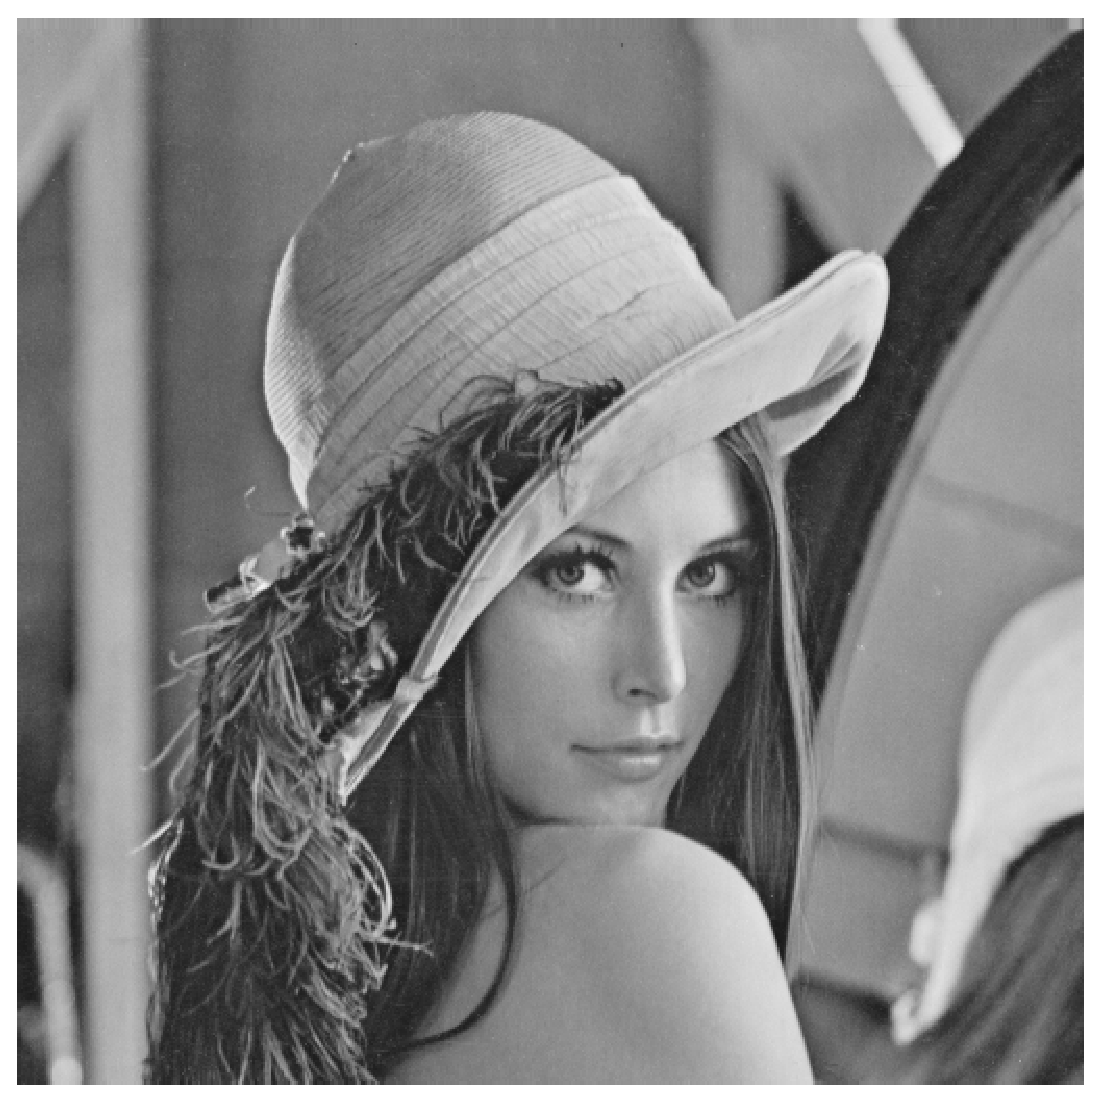
\includegraphics[width = 5 cm]{lena}
  \caption{Imagem-base para o processamento, popularmente conhecida como Lena. Fonte: fornecida pelo professor}
  \label{fig:lena}
\end{figure}

\begin{figure}[!t]
  \centering
  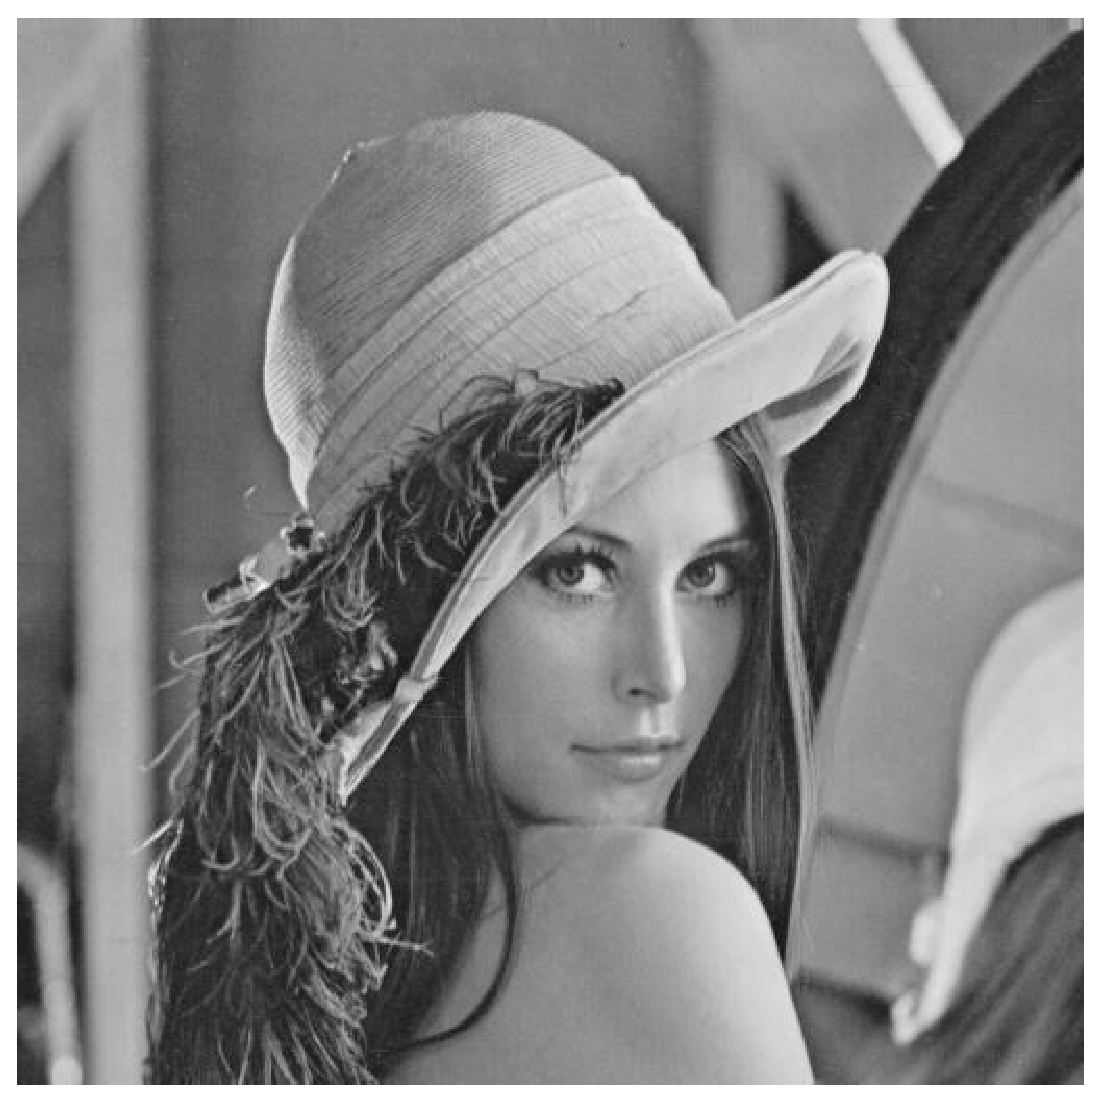
\includegraphics[width = 5 cm]{lena_1}
  \caption{Imagem reconstru\'ida a partir do passo de quantiza\c{c}\~ao 1.}
  \label{fig:lena1}
\end{figure}

\begin{figure}[!t]
  \centering
  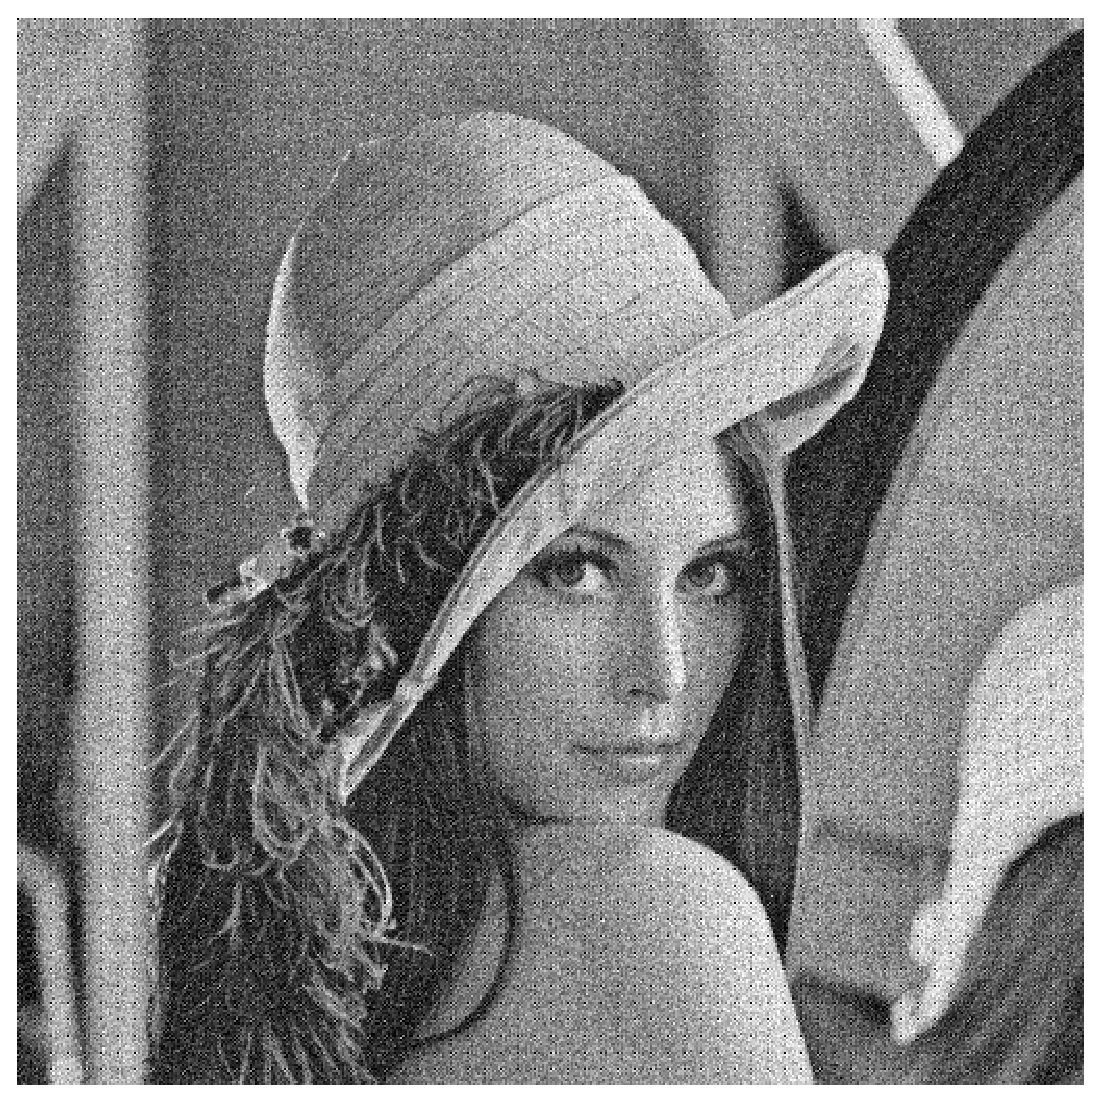
\includegraphics[width = 5 cm]{lena_50}
  \caption{Imagem reconstru\'ida a partir do passo de quantiza\c{c}\~ao 50.}
  \label{fig:lena50}
\end{figure}

A partir das reconstru\c{c}\~oes foi poss\'ivel construir a Figura~\ref{fig:psnrxvar}, que demostra a varia\c{c}\~ao da PSNR em fun\c{c}\~ao da Vari\^ancia. Al\'em disso, h\'a as Figuras~\ref{fig:psnr} e~\ref{fig:var} demonstram a varia\c{c}\~ao da PSNR e da Vari\^ancia em fun\c{c}\~ao do passo de quantiza\c{c}\~ao, respectivamente.

\begin{figure}[!t]
  \centering
  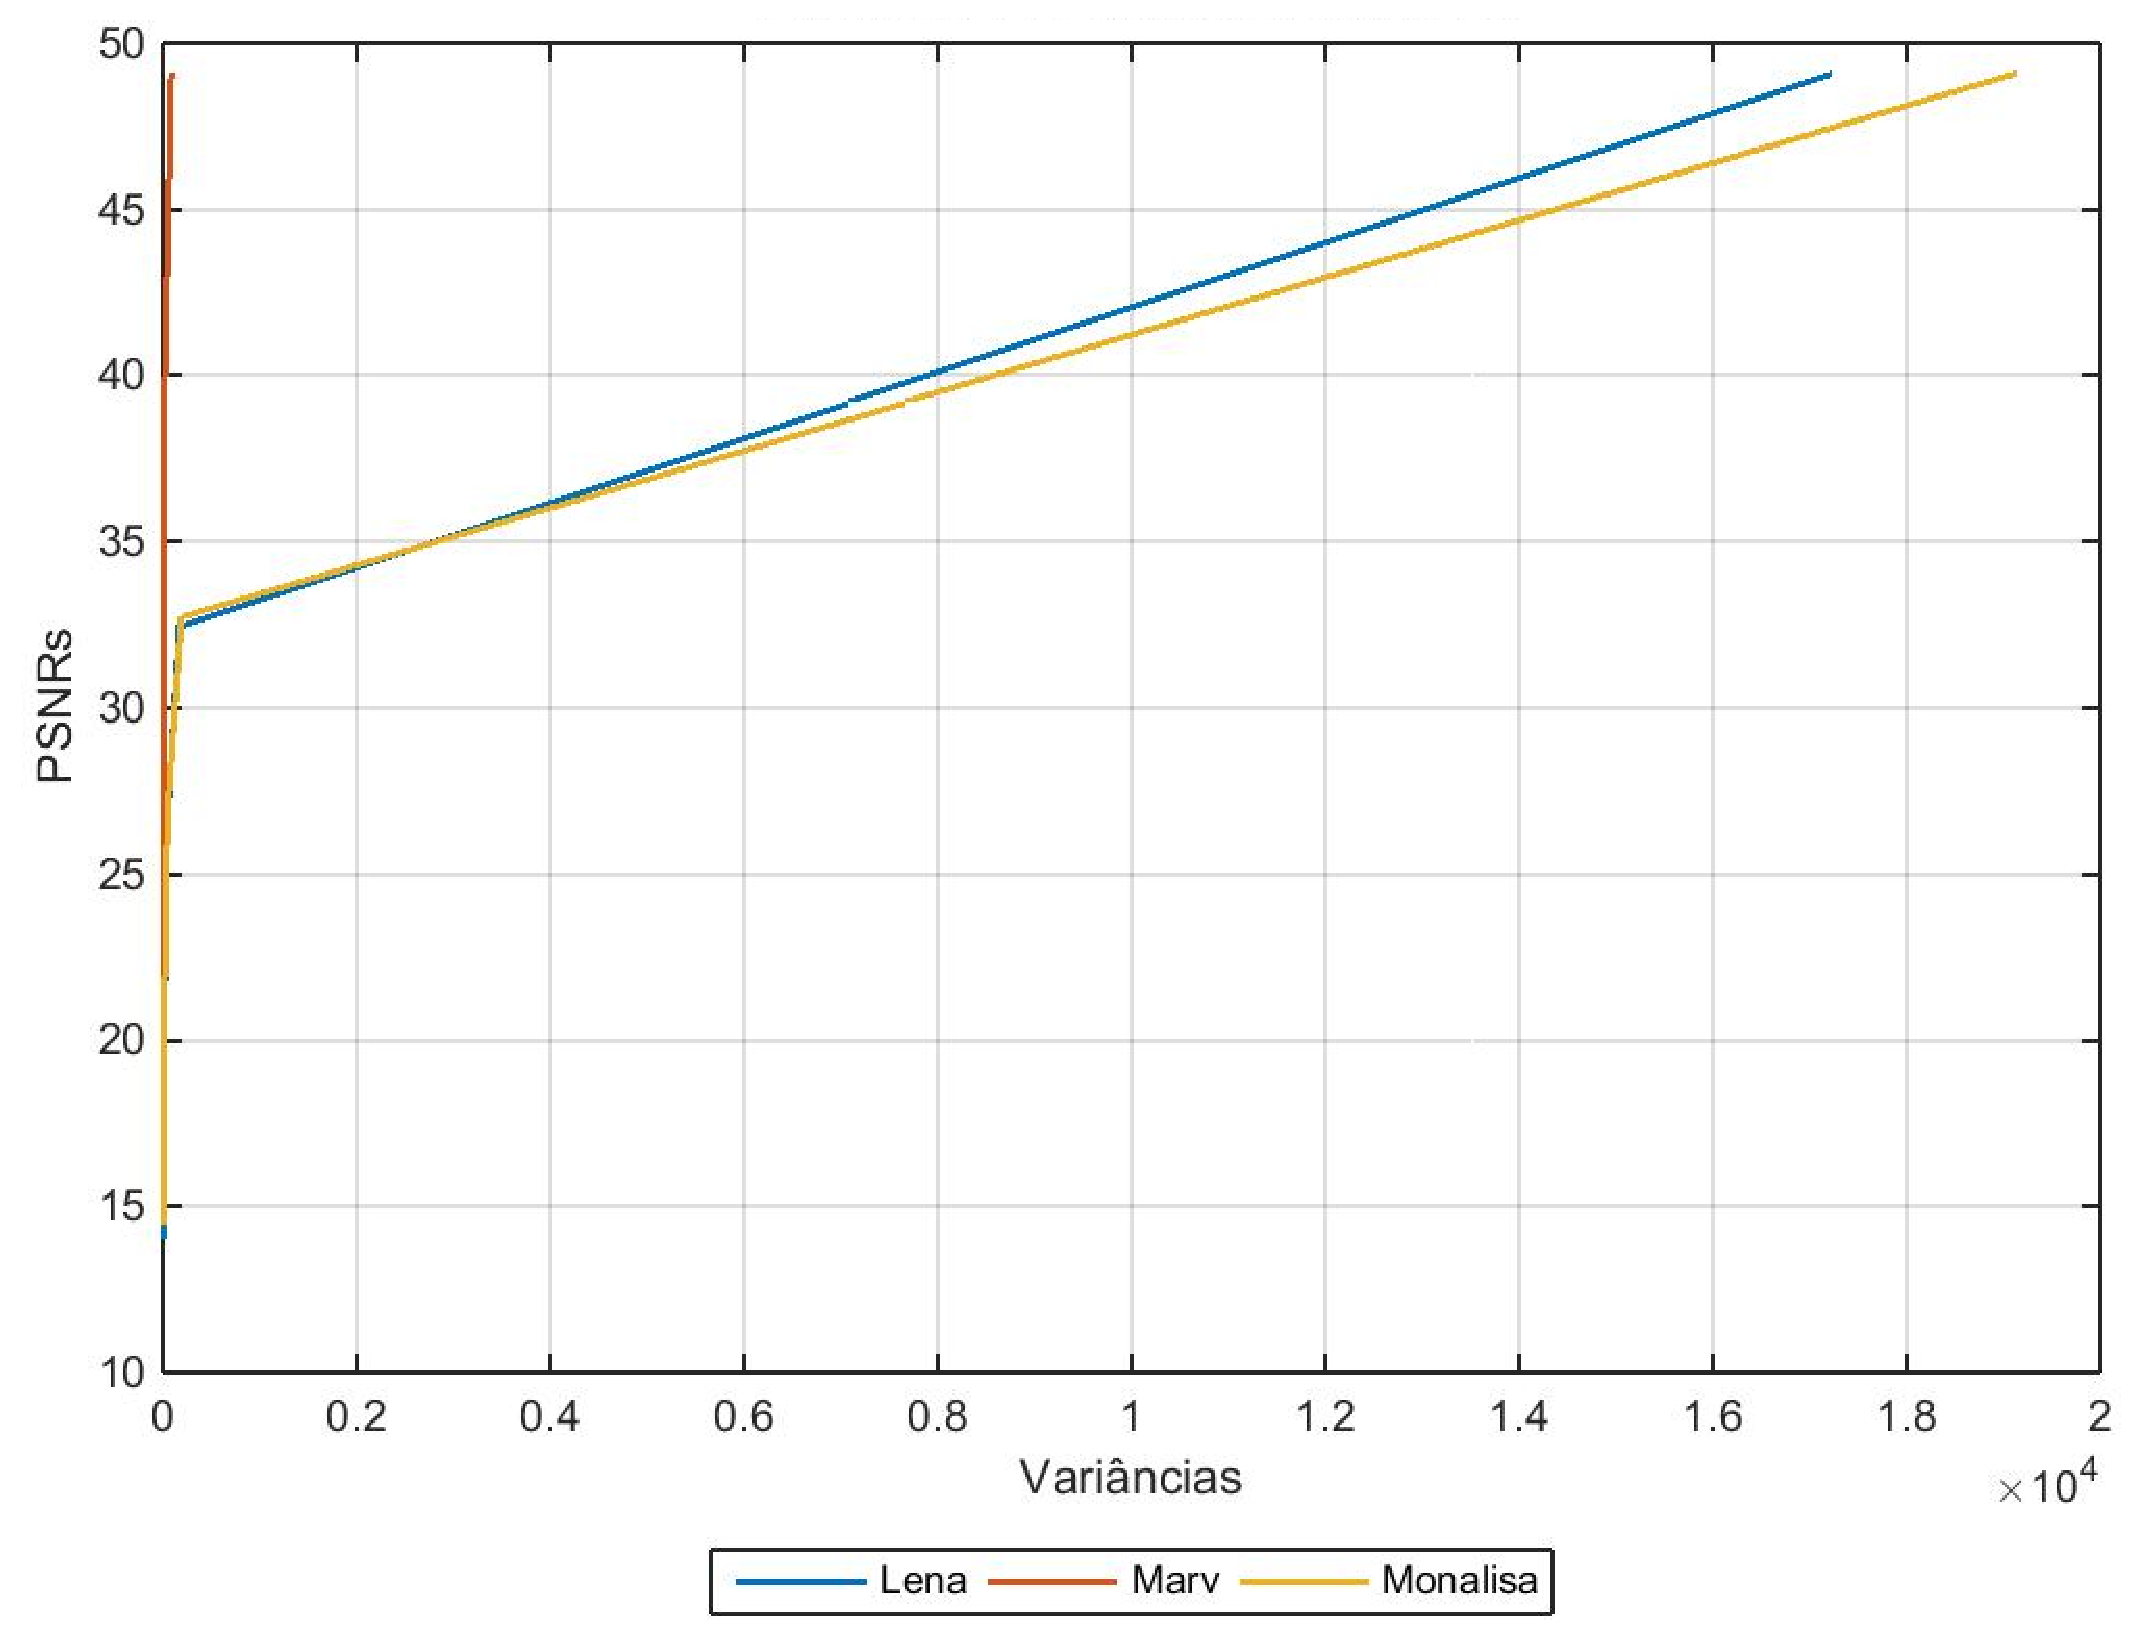
\includegraphics[width = 6.5 cm]{psnrxvar}
  \caption{Varia\c{c}\~ao das PSNR dado as Vari\^ancias.}
  \label{fig:psnrxvar}
\end{figure}

\begin{figure}[!t]
  \centering
  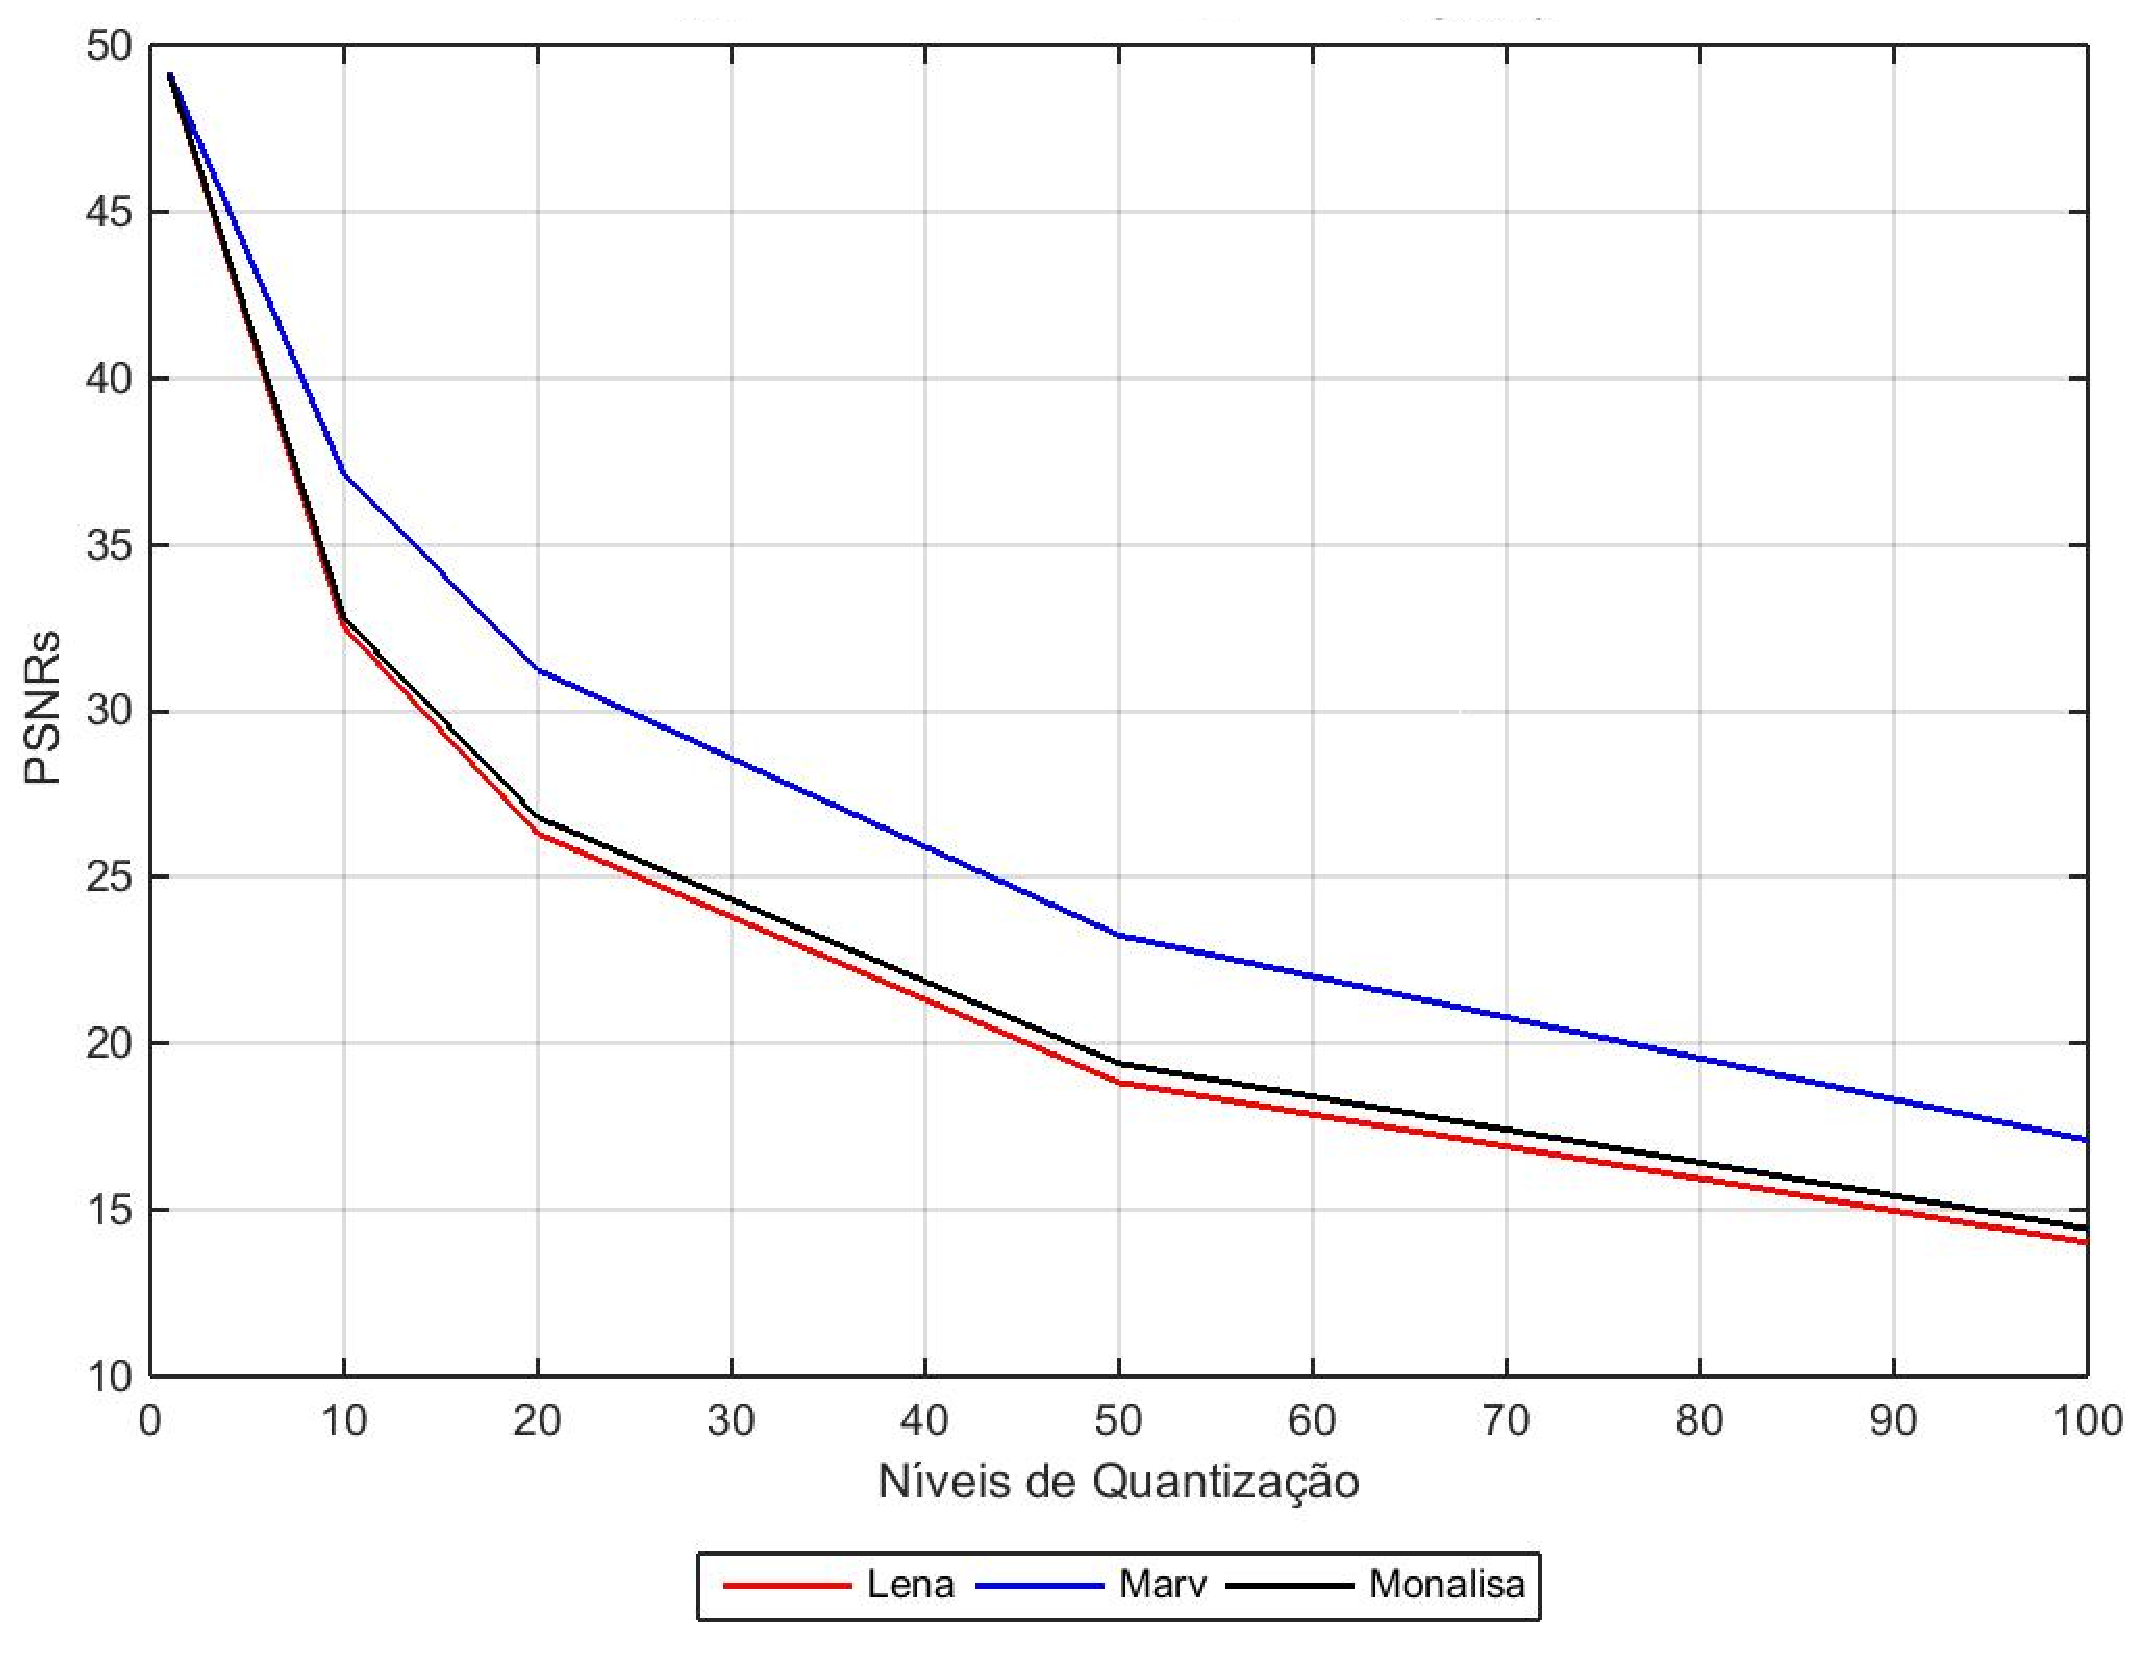
\includegraphics[width = 6.5 cm]{psnr}
  \caption{Varia\c{c}\~ao das PSNR das tr\^es imagens-base com suas respectivas reconstru\'idas, dado um n\'ivel de quantiza\c{c}\~ao.}
  \label{fig:psnr}
\end{figure}

\begin{figure}[!t]
  \centering
  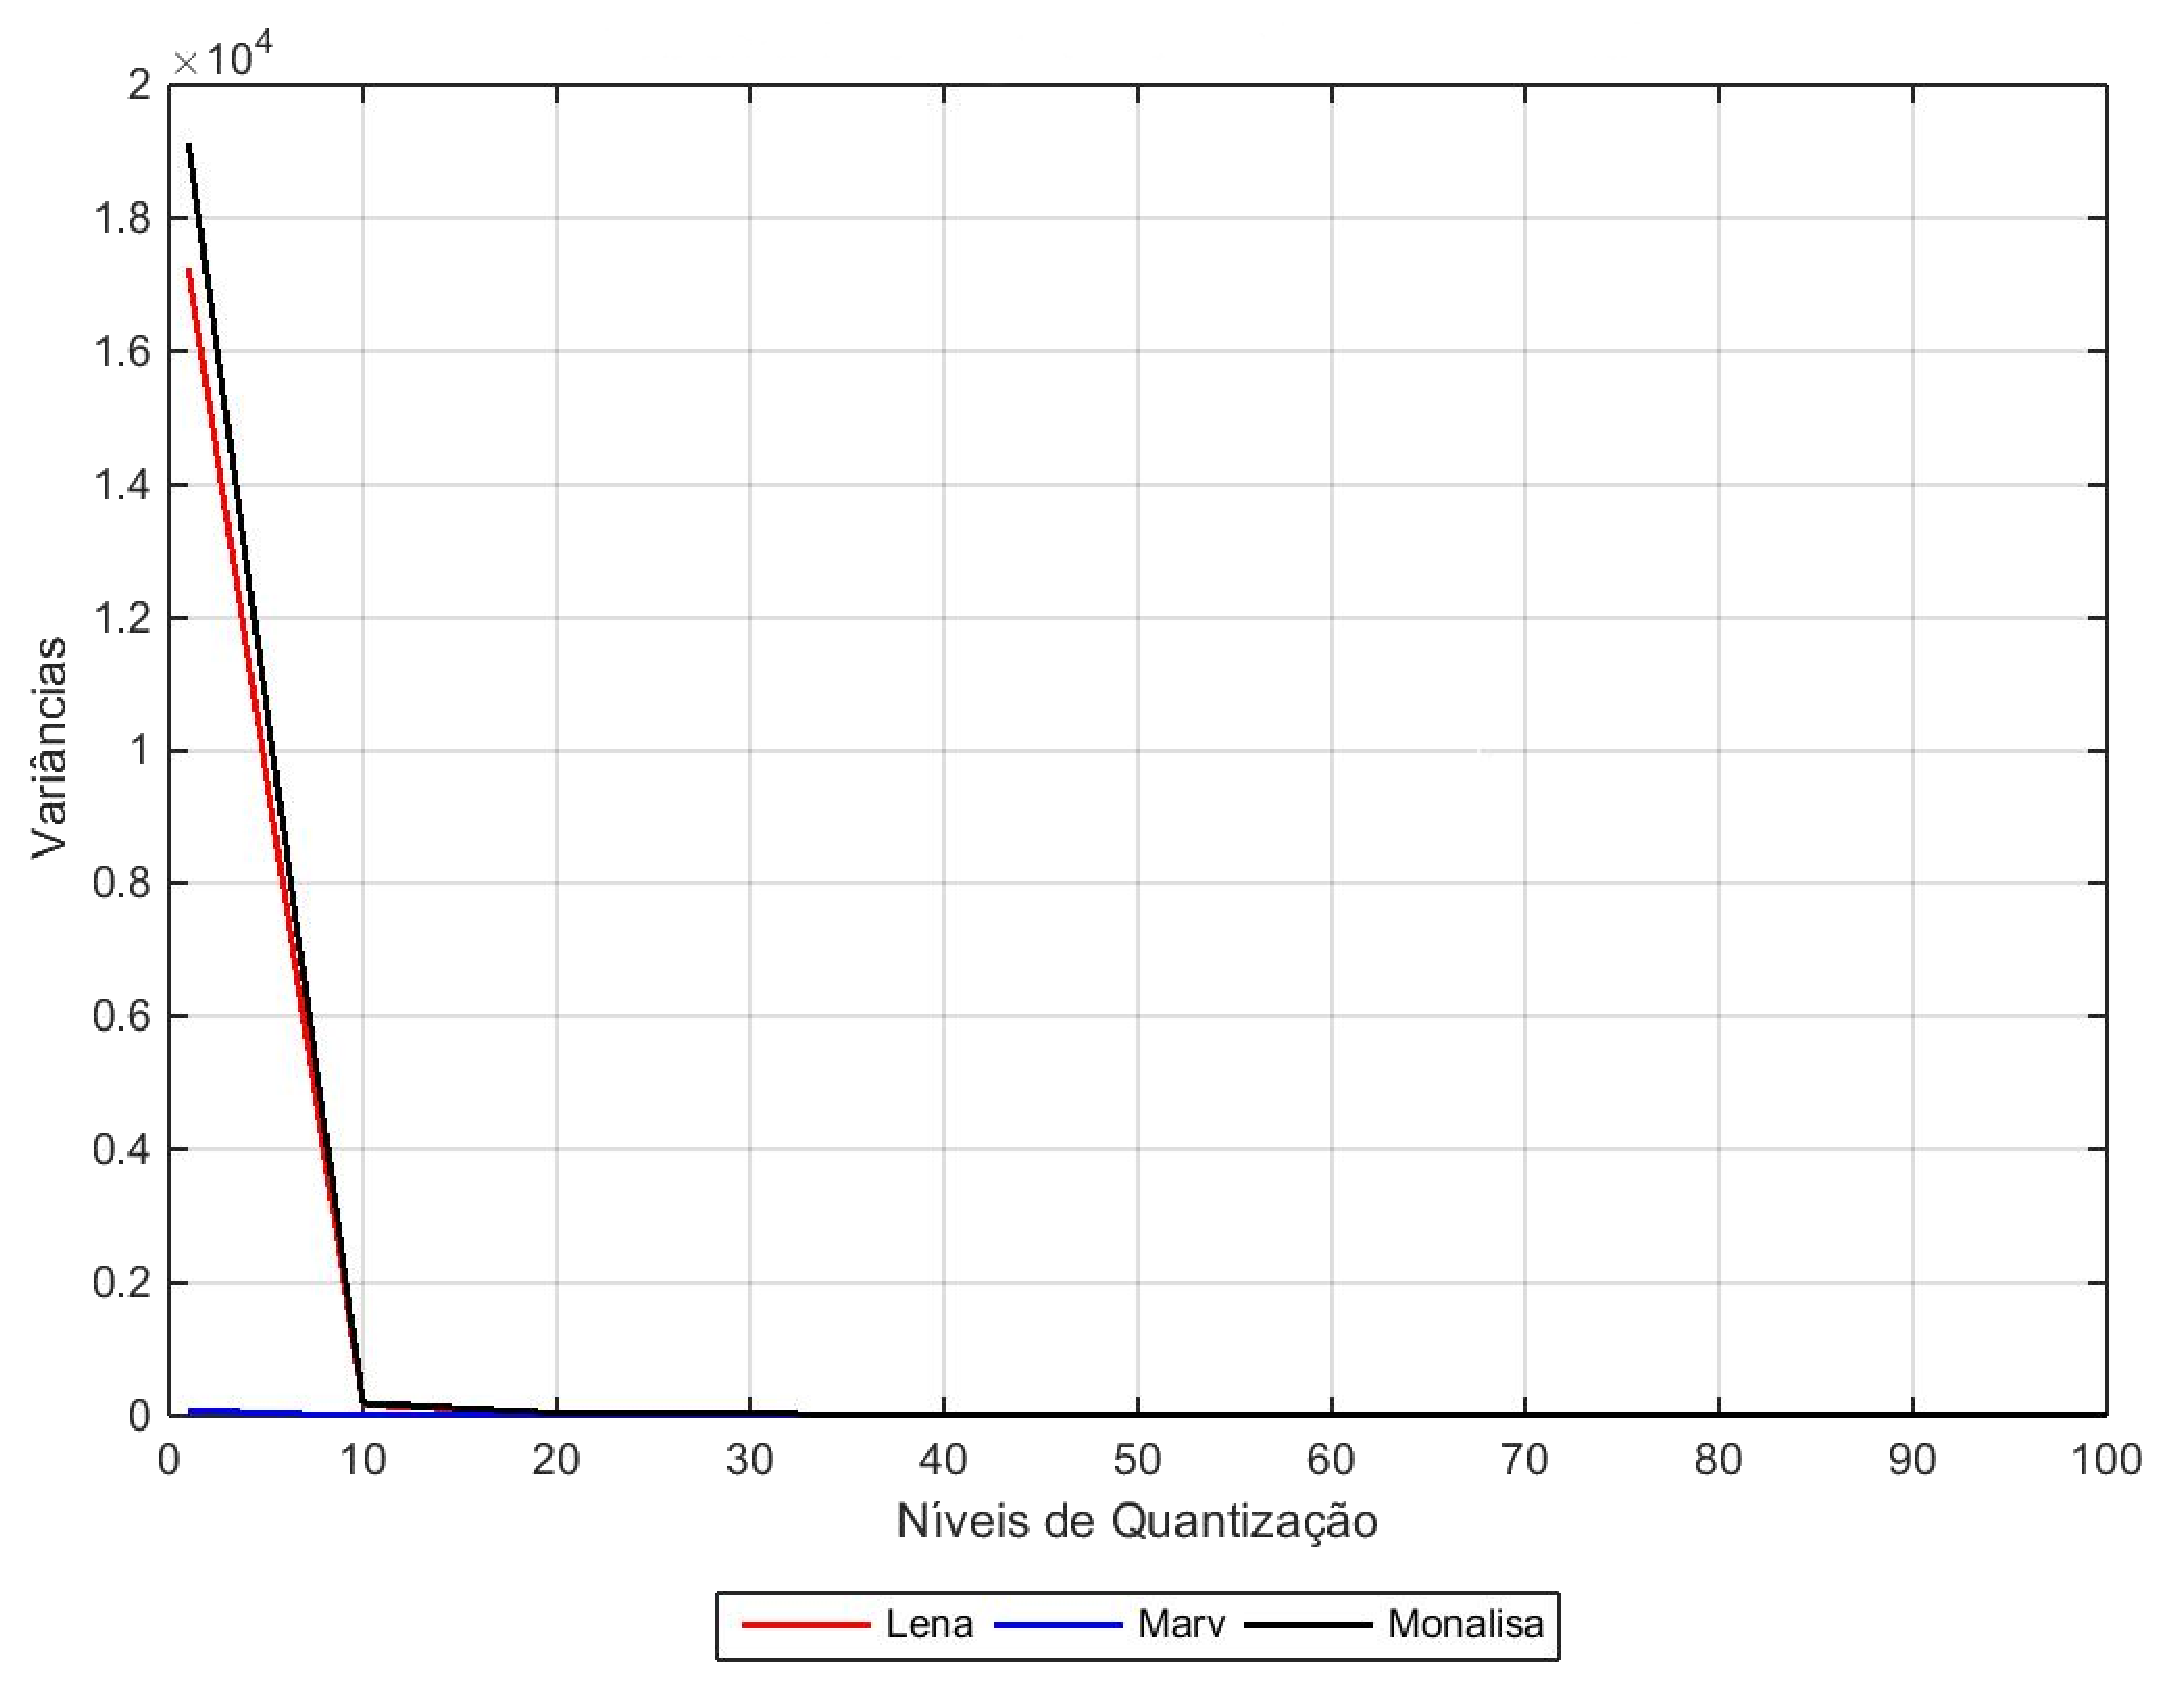
\includegraphics[width = 6.5 cm]{var}
  \caption{Varia\c{c}\~ao das Vari\^ancias das tr\^es imagens-base com suas respectivas reconstru\'idas, dado um n\'ivel de quantiza\c{c}\~ao.}
  \label{fig:var}
\end{figure}

%%%%%%%%%%%%%%%%%%%%%%%%%%%%%%%%%%%%%%%
\subsection{DPCM antes da Codifica\c{c}\~ao}
  \label{dpcmlossy_metodo}
%%%%%%%%%%%%%%%%%%%%%%%%%%%%%%%%%%%%%%%
Foi escolhido mostrar os resultados sobre a Figura~\ref{fig:lena}, onde para esta tem-se: Figura~\ref{fig:lena1_2} que demostra a imagem reconstru\'ida a partir do passo de quantiza\c{c}\~ao 1, que obteve um PSNR de $10.47 db$; enquanto que para a Figura~\ref{fig:lena50_2} foi aplicado o passo de quantiza\c{c}\~ao 50, que obteve um PSNR de $10.40 db$.

\begin{figure}[!t]
  \centering
  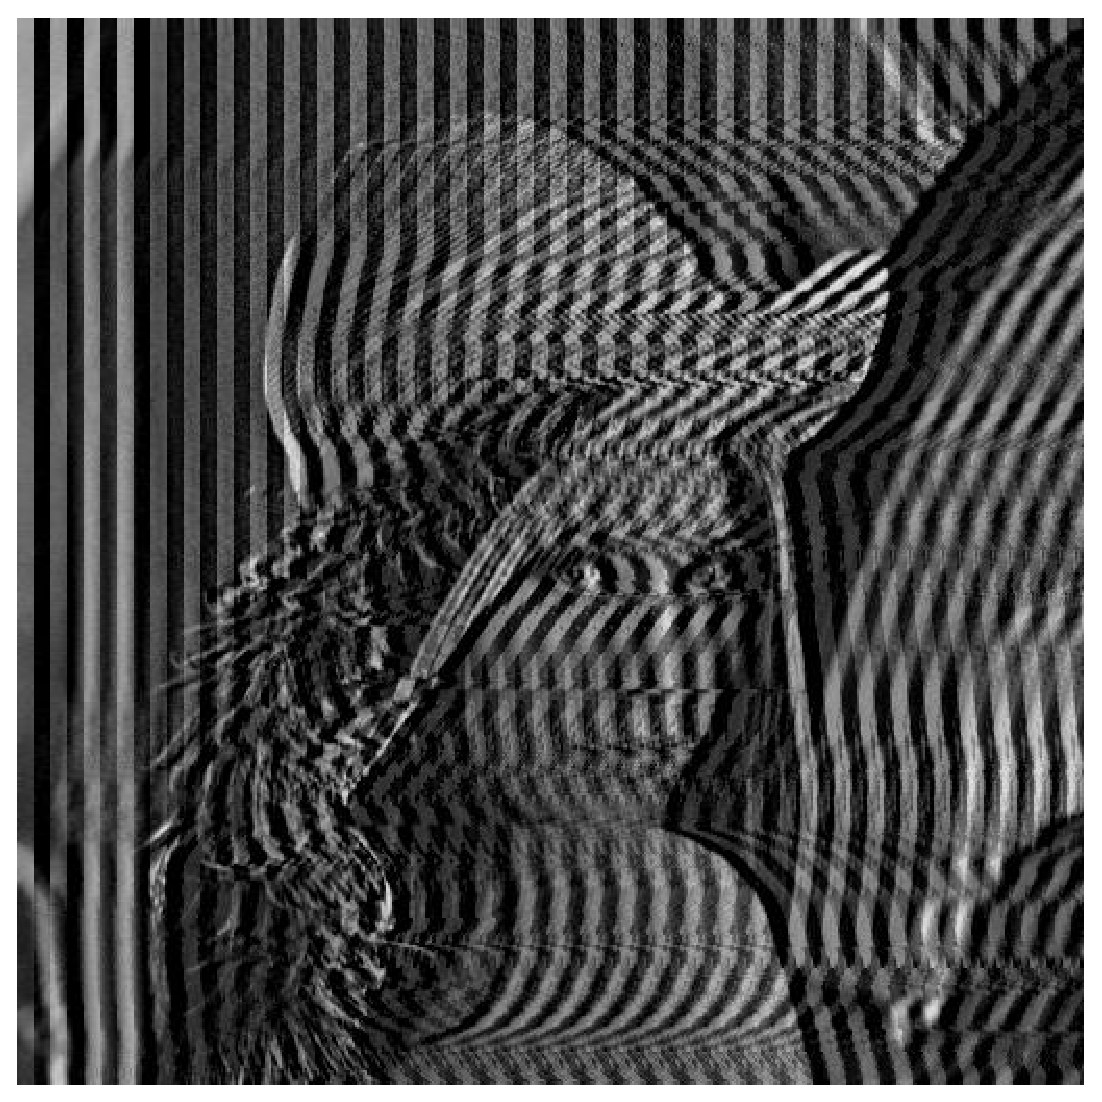
\includegraphics[width = 5 cm]{lena_1_2}
  \caption{Imagem reconstru\'ida a partir do passo de quantiza\c{c}\~ao 1, sendo aplicado o DPCM antes da codifica\c{c}\~ao.}
  \label{fig:lena1_2}
\end{figure}

\begin{figure}[!t]
  \centering
  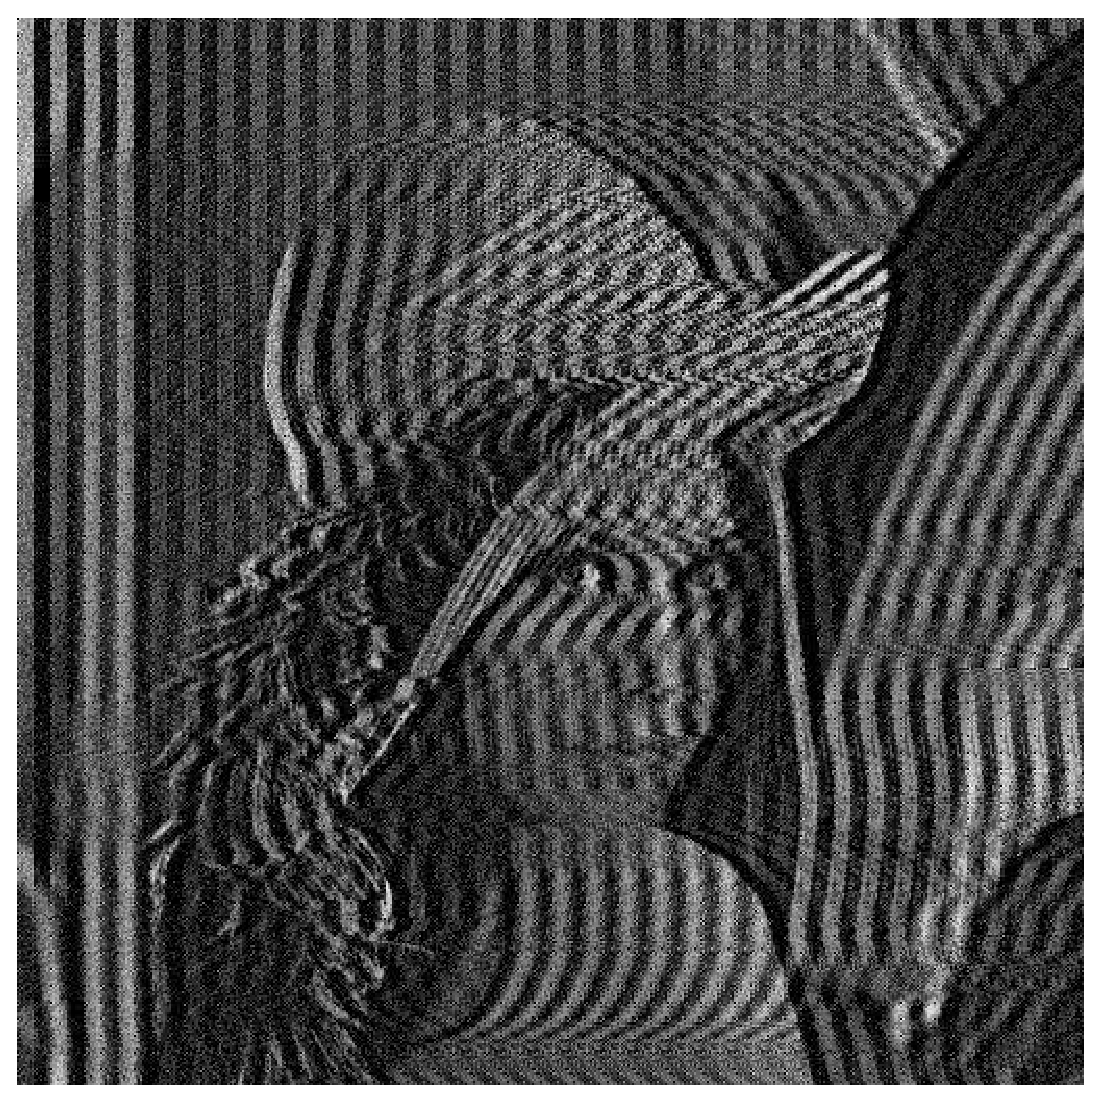
\includegraphics[width = 5 cm]{lena_50_2}
  \caption{Imagem reconstru\'ida a partir do passo de quantiza\c{c}\~ao 50, sendo aplicado o DPCM antes da codifica\c{c}\~ao.}
  \label{fig:lena50_2}
\end{figure}

A partir das reconstru\c{c}\~oes foi poss\'ivel construir a Figura~\ref{fig:psnrxvar_2}, que demostra a varia\c{c}\~ao da PSNR em fun\c{c}\~ao da Vari\^ancia. Al\'em disso, h\'a as Figuras~\ref{fig:psnr_2} e~\ref{fig:var_2} demonstram a varia\c{c}\~ao da PSNR e da Vari\^ancia em fun\c{c}\~ao do passo de quantiza\c{c}\~ao, respectivamente.

\begin{figure}[!t]
  \centering
  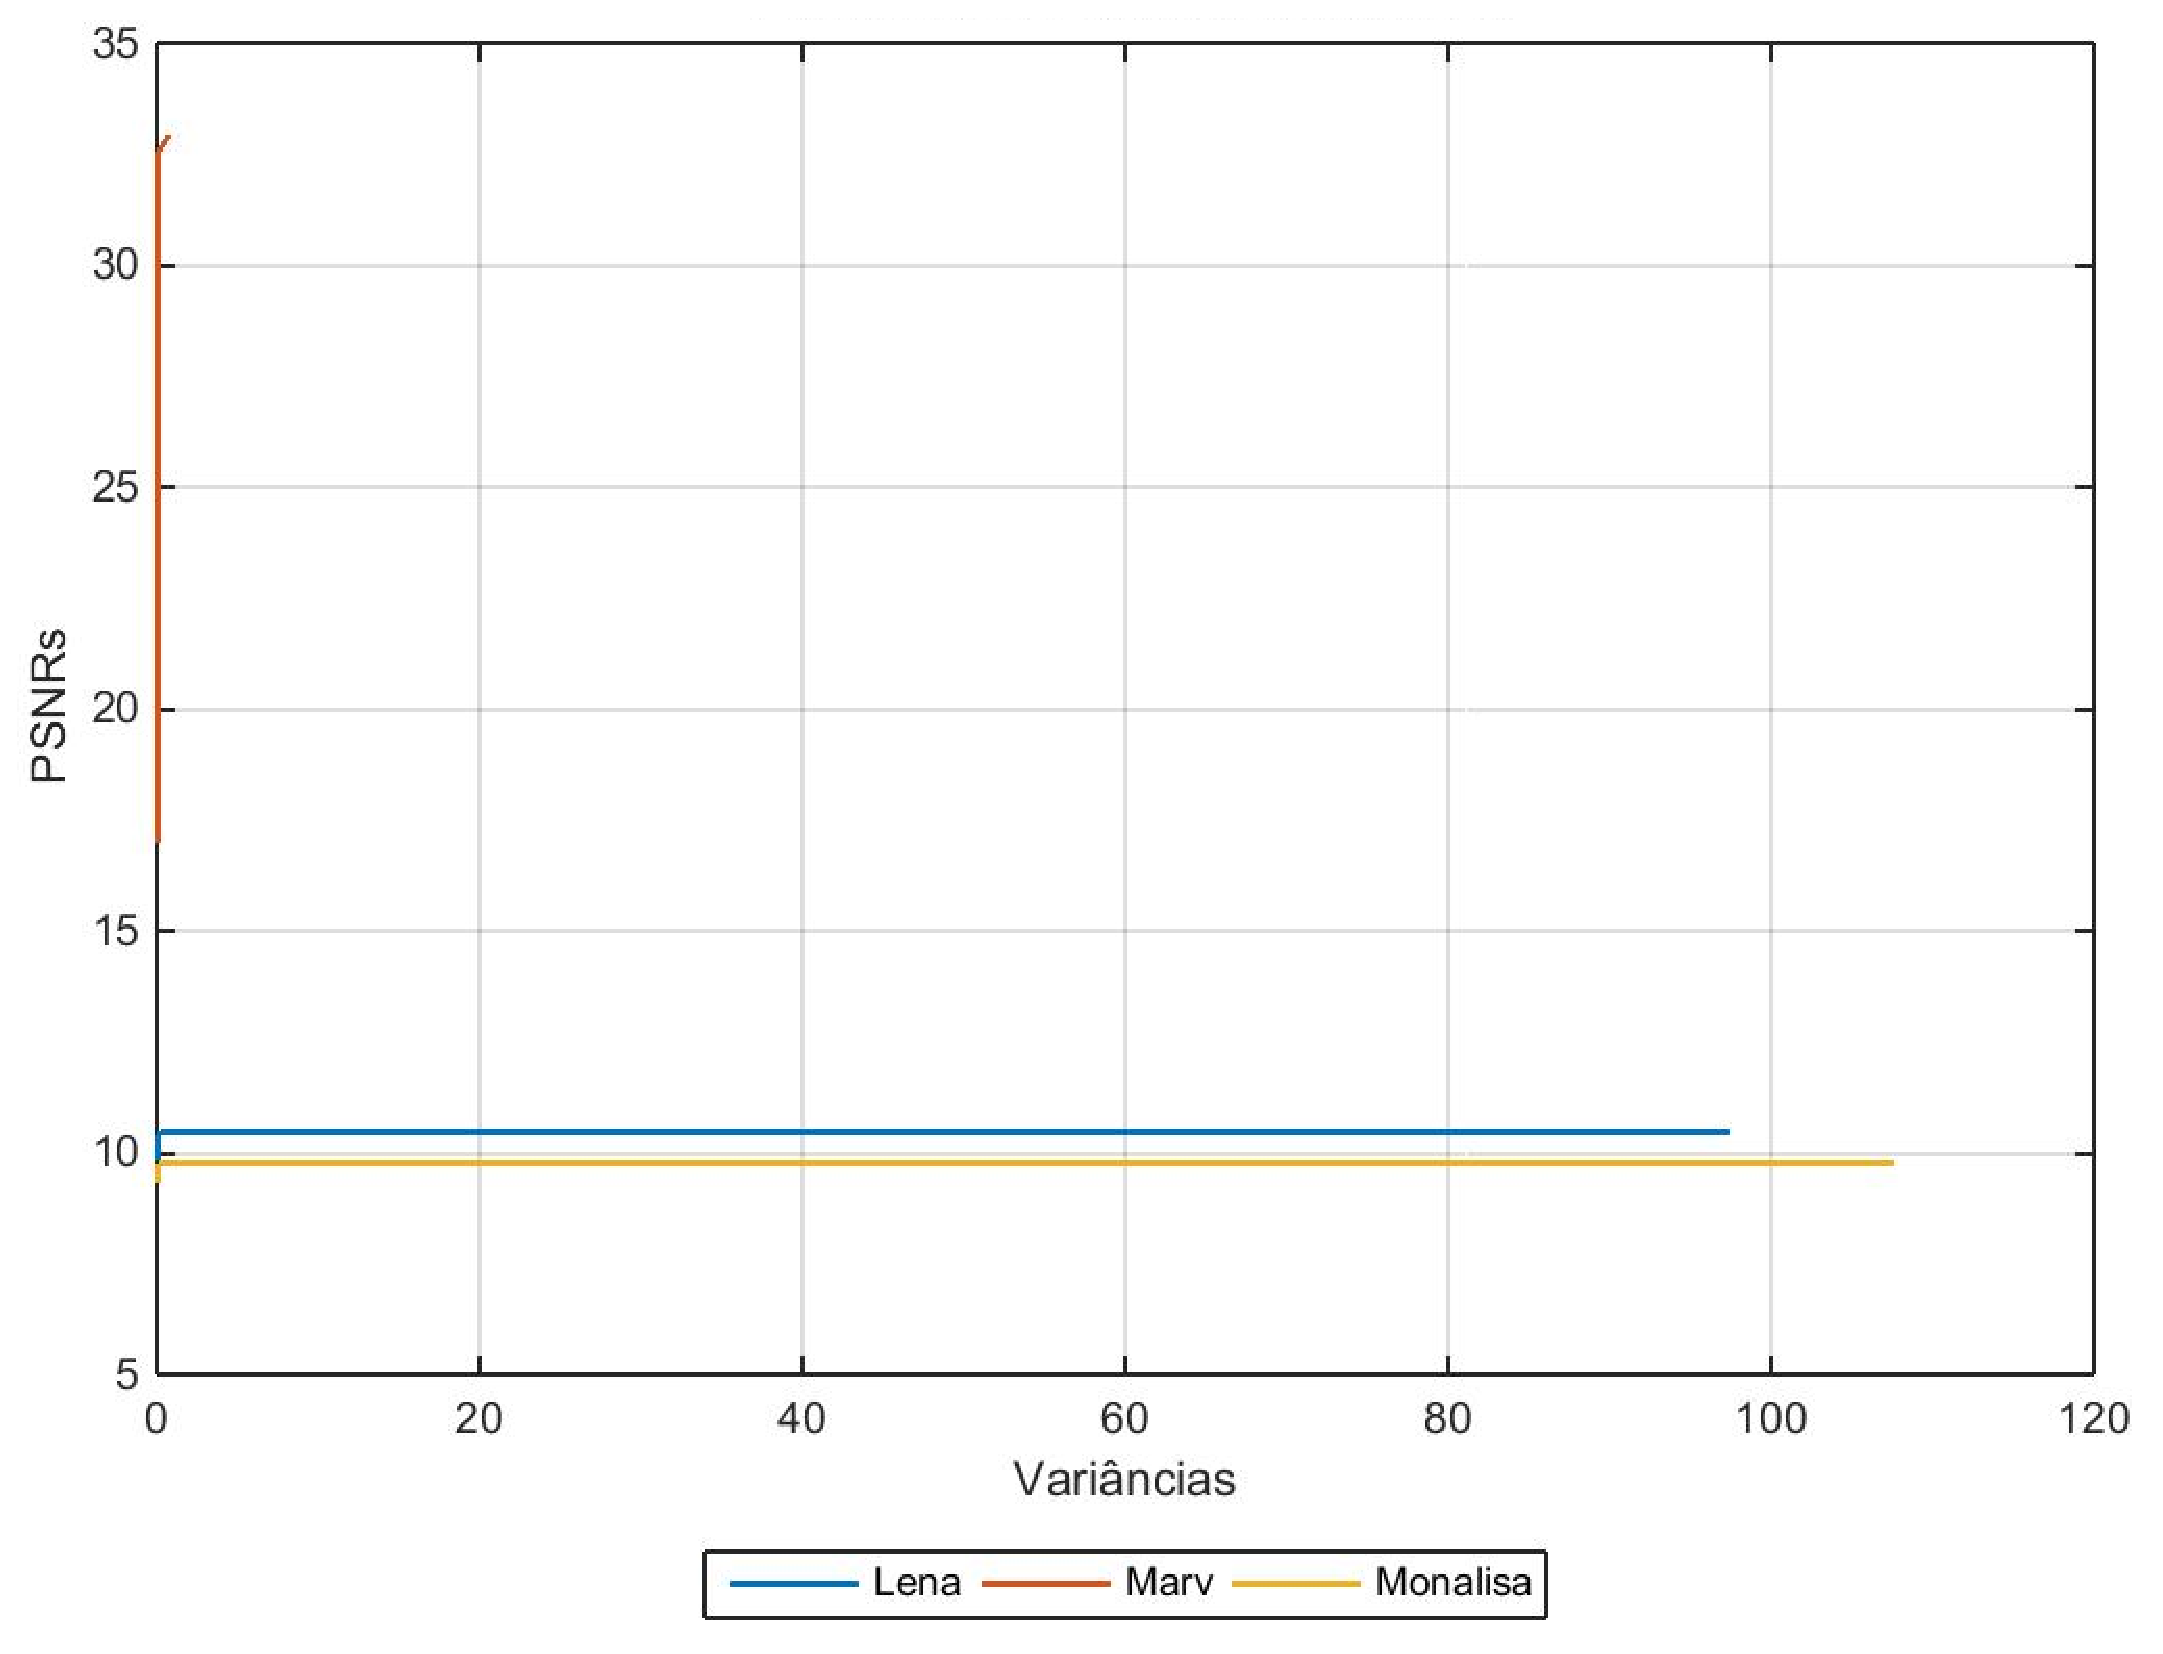
\includegraphics[width = 6.5 cm]{psnrxvar_2}
  \caption{Varia\c{c}\~ao das PSNR dado as Vari\^ancias, com DPCM antes da codifica\c{c}\~ao.}
  \label{fig:psnrxvar_2}
\end{figure}

\begin{figure}[!t]
  \centering
  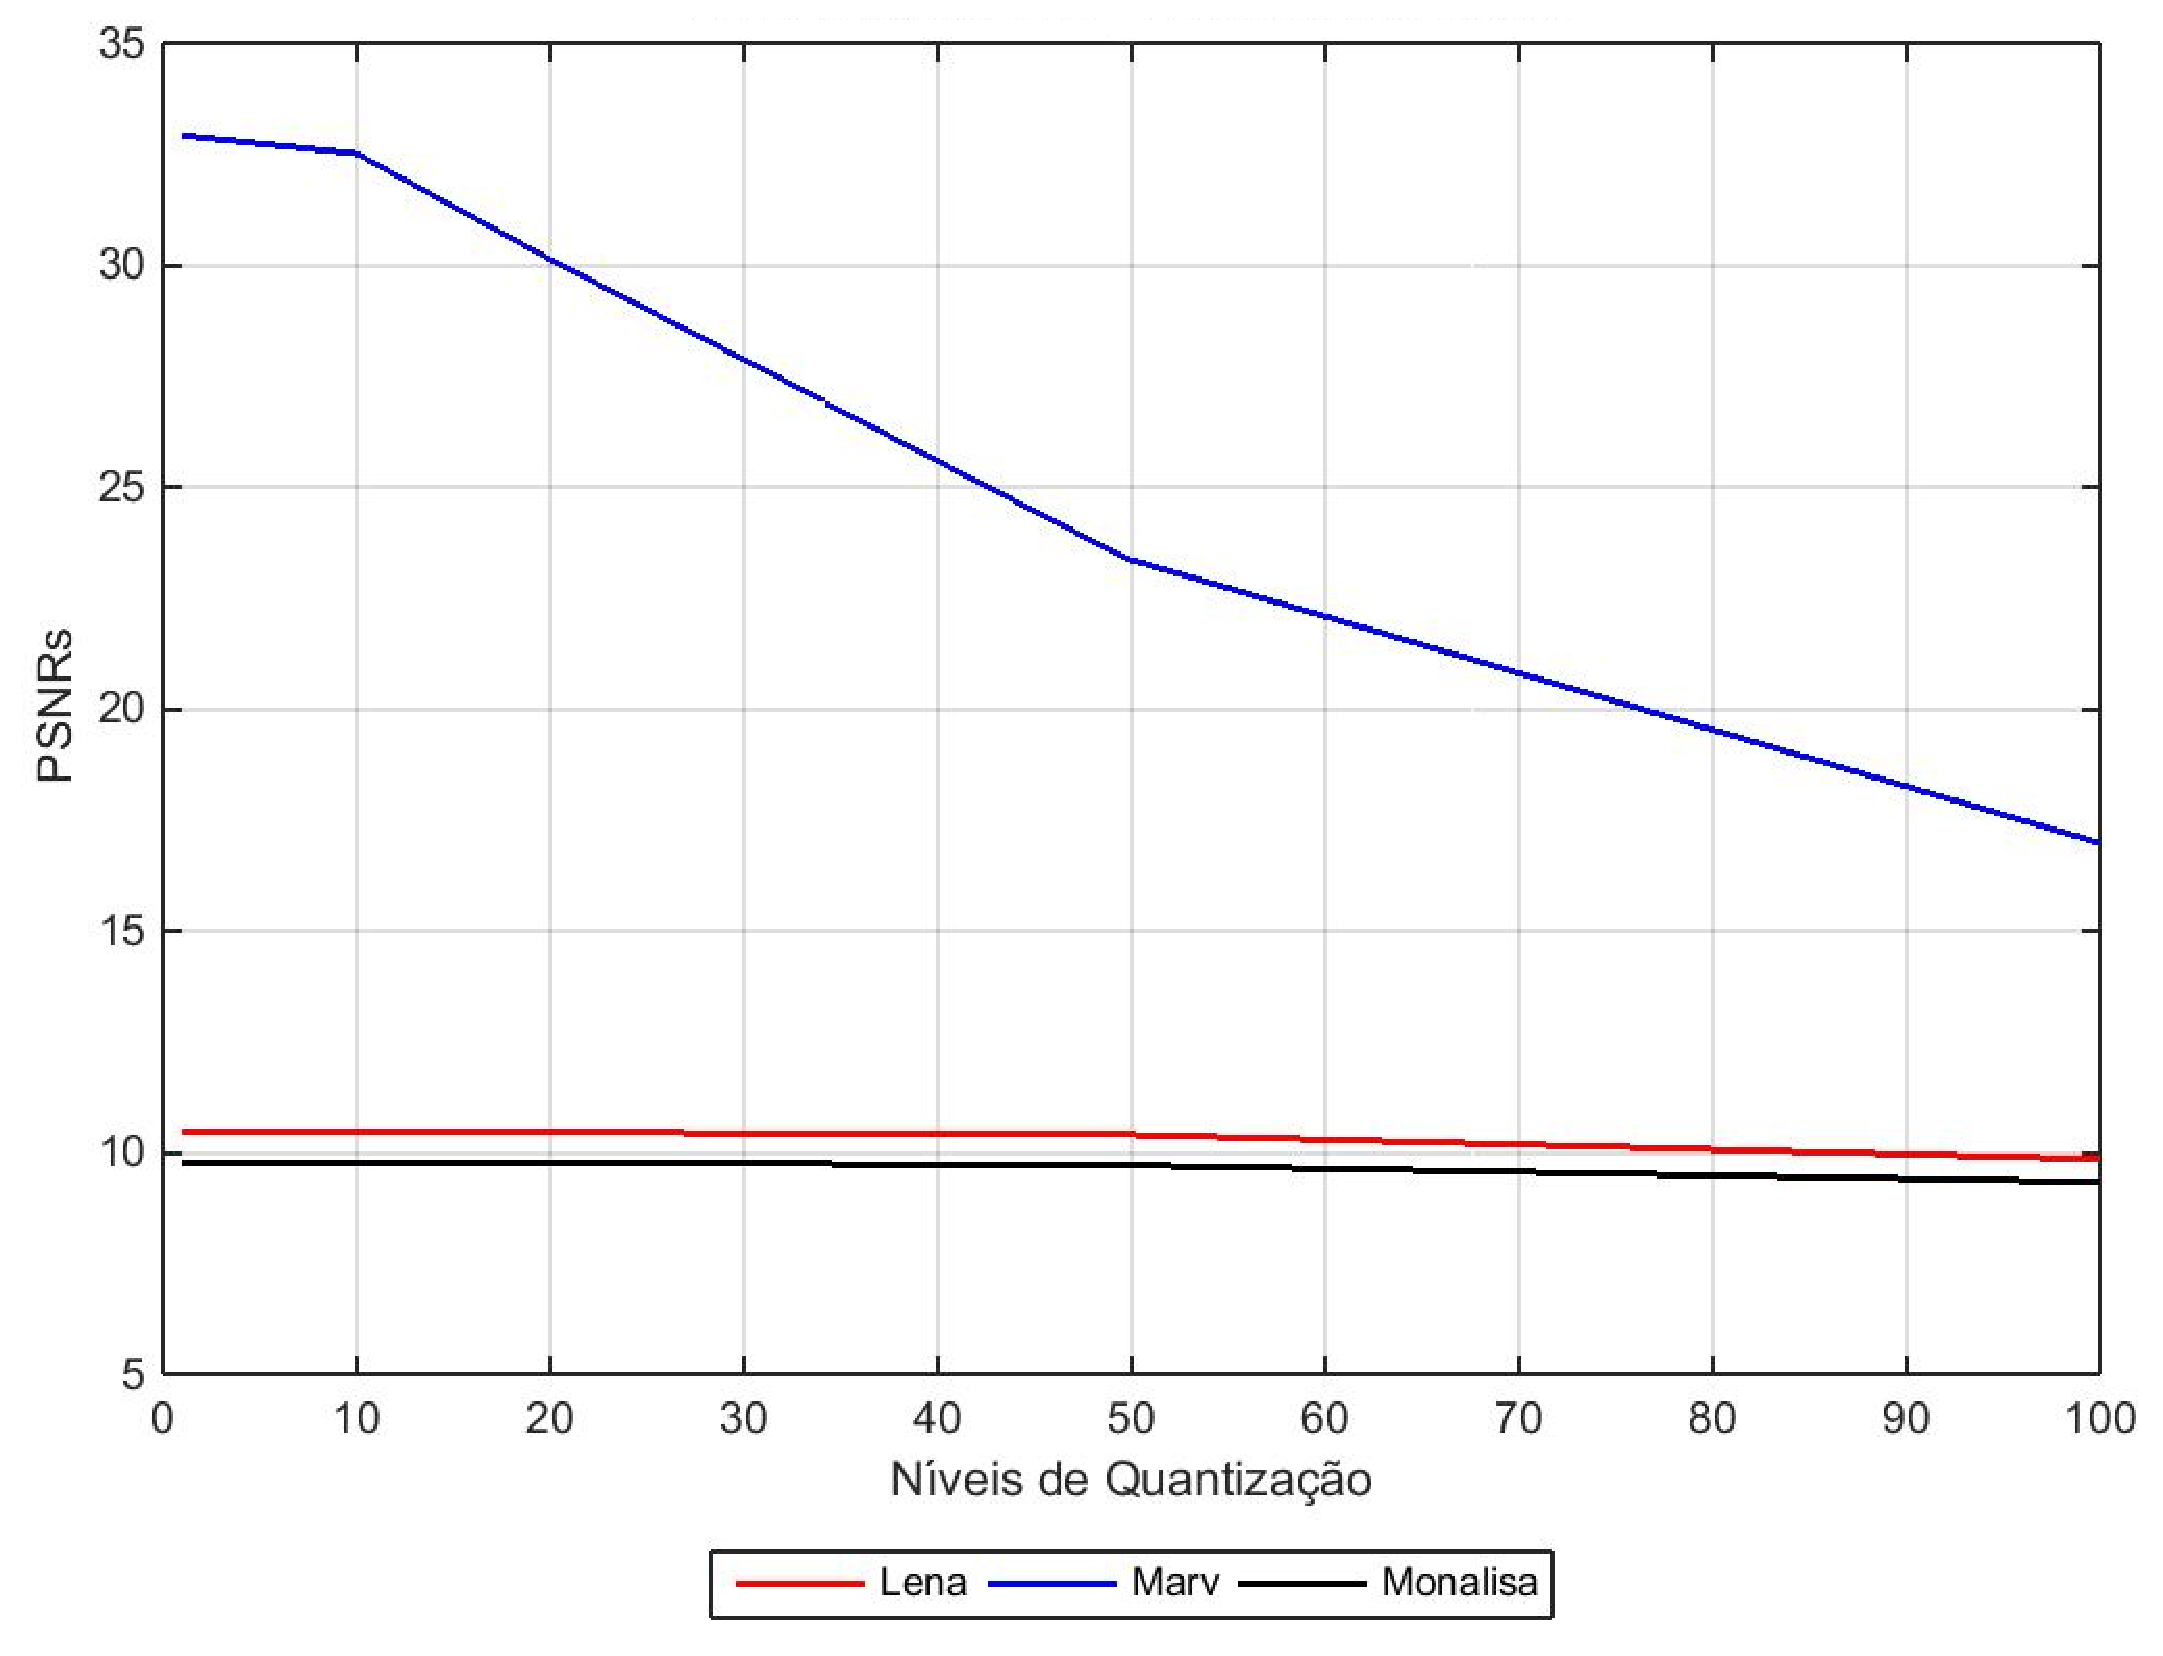
\includegraphics[width = 6.5 cm]{psnr_2}
  \caption{Varia\c{c}\~ao das PSNR das tr\^es imagens-base com suas respectivas reconstru\'idas, dado um n\'ivel de quantiza\c{c}\~ao, com DPCM antes da codifica\c{c}\~ao.}
  \label{fig:psnr_2}
\end{figure}

\begin{figure}[!t]
  \centering
  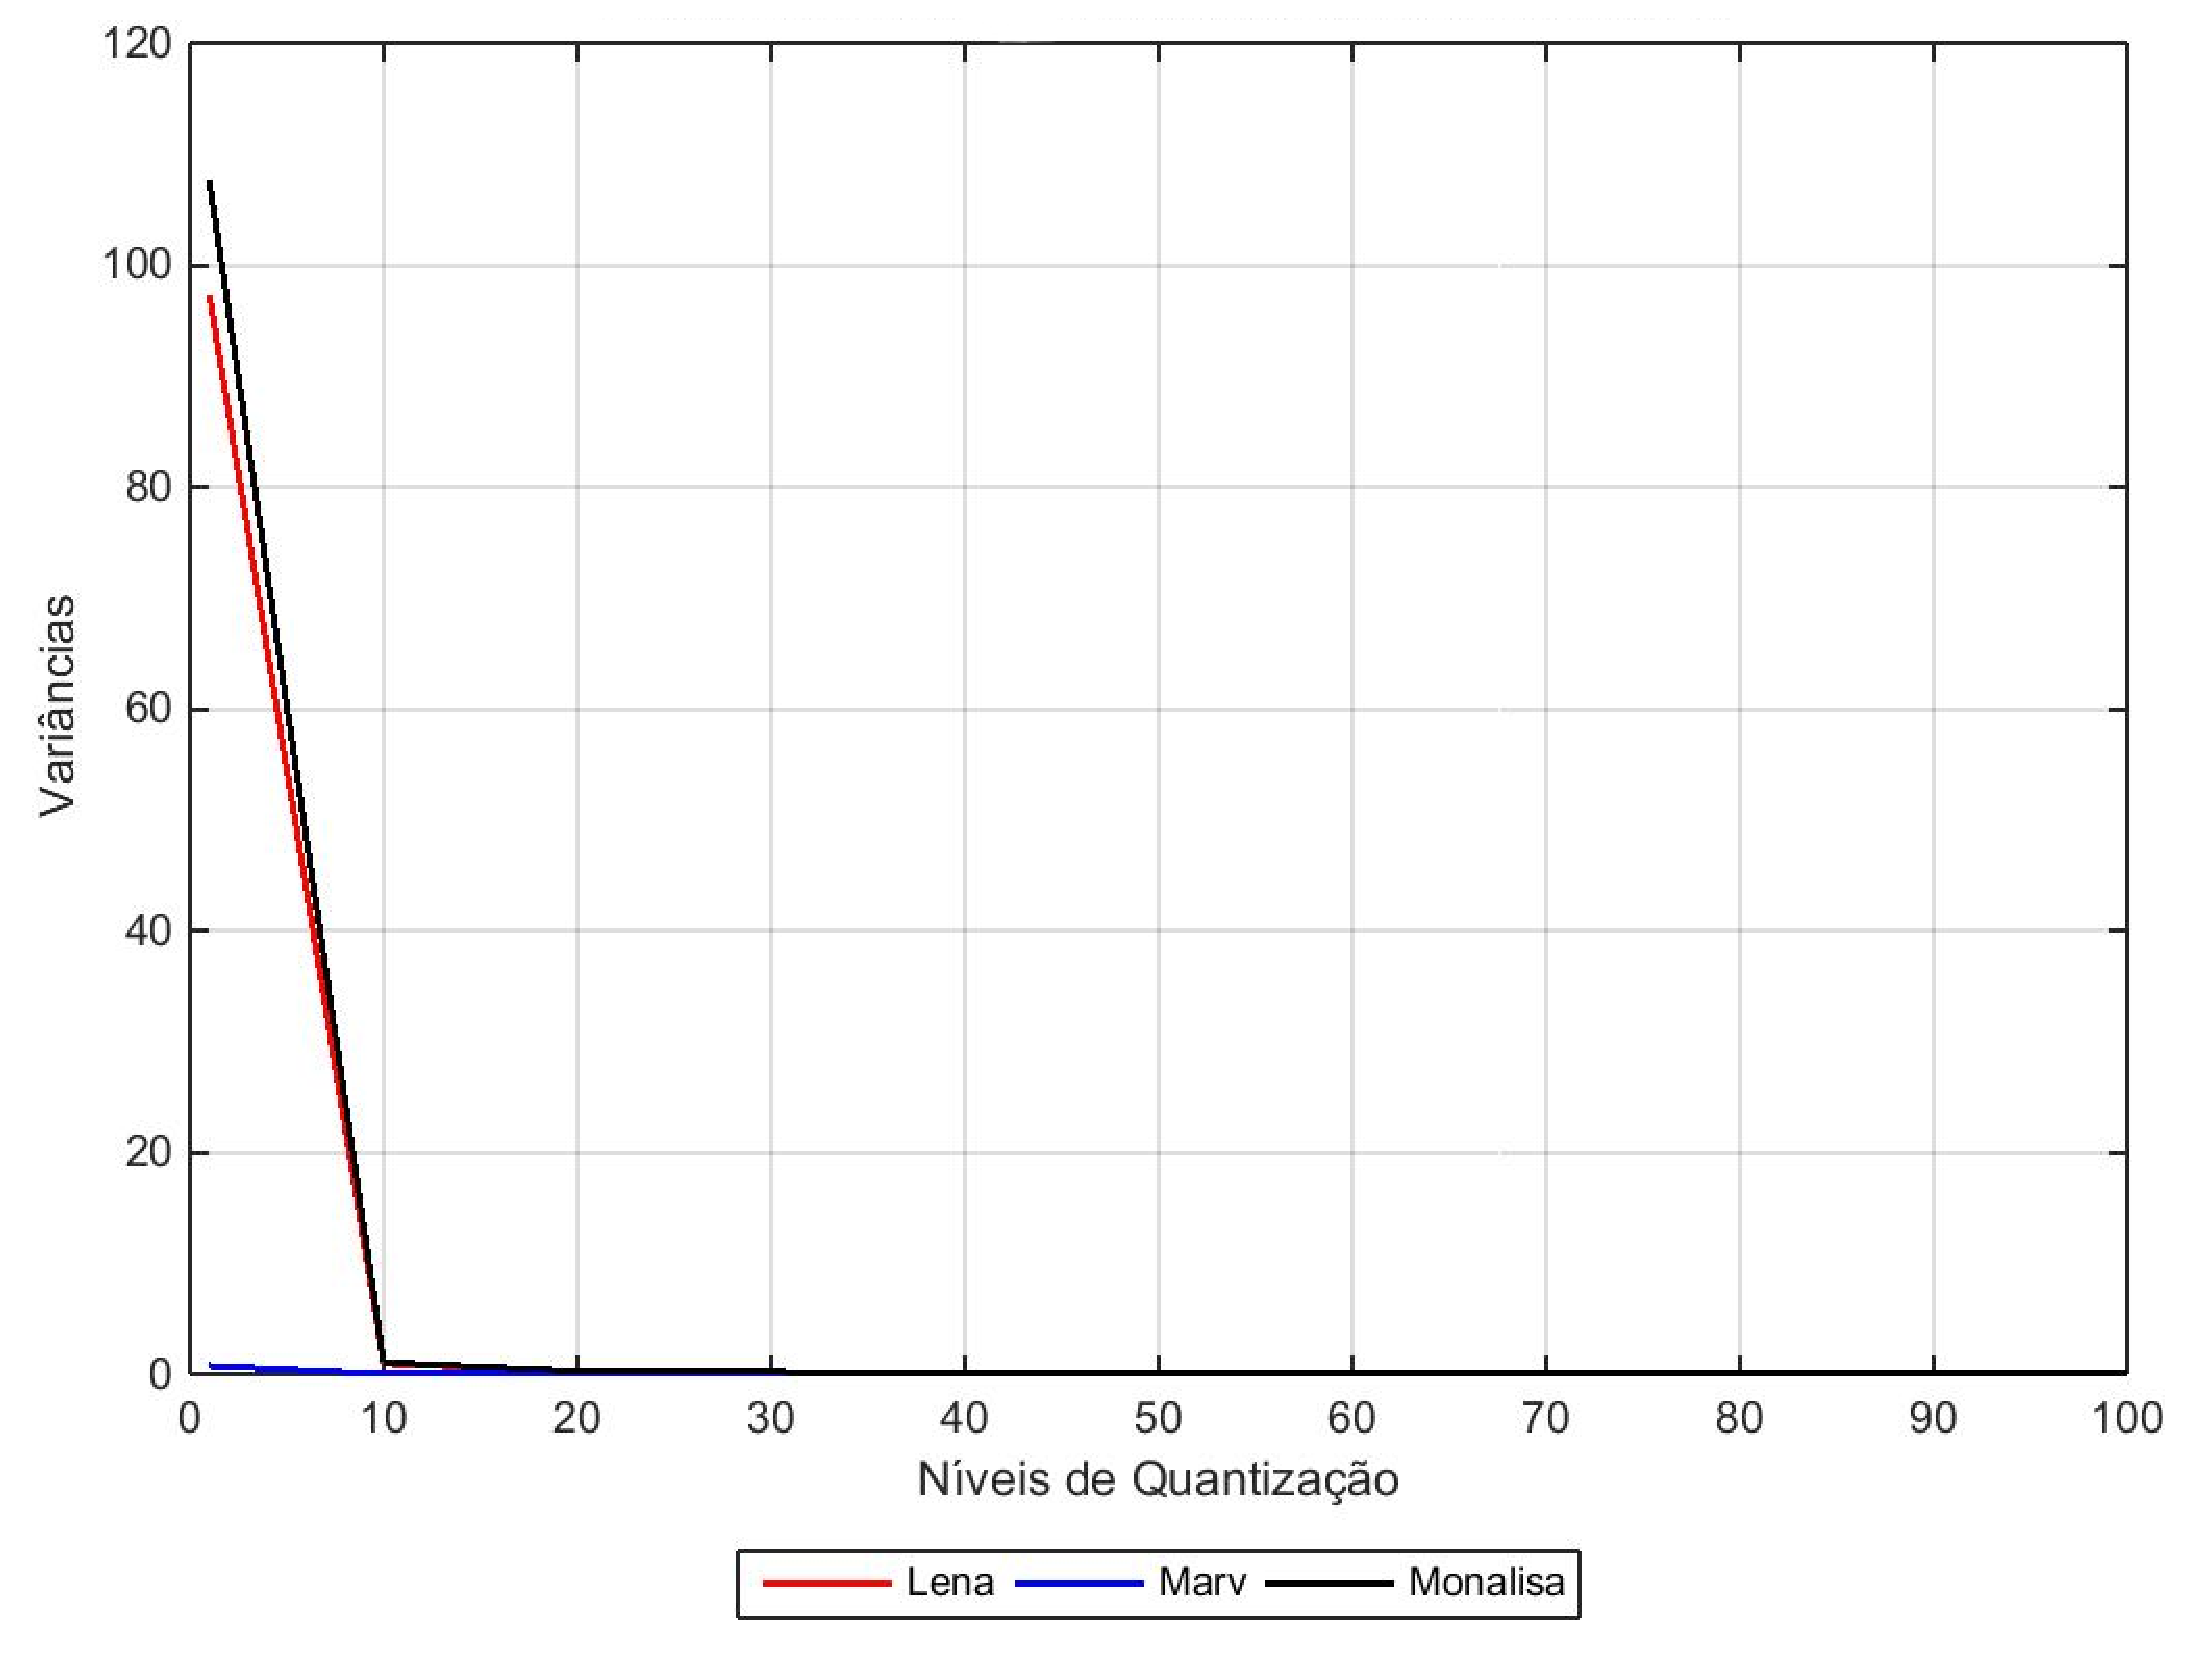
\includegraphics[width = 6.5 cm]{var_2}
  \caption{Varia\c{c}\~ao das Vari\^ancias das tr\^es imagens-base com suas respectivas reconstru\'idas, dado um n\'ivel de quantiza\c{c}\~ao, com DPCM antes da codifica\c{c}\~ao.}
  \label{fig:var_2}
\end{figure}


%%%%%%%%%%%%%%%%%%%%%%%%%%%%%%%%%%%%%%%%%%%%%%%%%%%%%%%%%%%%%%%%%%%%%%%%%%%%%
\section{Conclus\~ao}
  \label{conclusao}
%%%%%%%%%%%%%%%%%%%%%%%%%%%%%%%%%%%%%%%%%%%%%%%%%%%%%%%%%%%%%%%%%%%%%%%%%%%%%
Com o desenvolvimento do projeto foi poss\'ivel sanar algunas d\'uvidas perante os conte\'udos te\'oricos visto em sala, demonstrando que o objetivo principal foi alcan\c{c}ado. Foram utilizadas as ferramentas disponibilizadas pelo~\textit{MatLab}, que possuem grande poder de atua\c{c}\~ao no processamento de imagens, o que facilitou a fixa\c{c}\~ao dos conceitos, mas \'e esperado que futuramente seja feita uma aplica\c{c}\~ao em~\textit{OpenCV}~\cite{opencv}~(\textit{Open Source Computer Vision Library} ou, em portugu\^es, Biblioteca de Vis\~ao Computacional em C\'odigo Aberto).

Ao analisar o primeiro problema foi observado que as imagens reconstru\'idas a partir de um passo de quantiza\c{c}\~ao maior eram tanto visualmente quanto pelo PSNR menos parecidas com as imagens originais, refor\c{c}ando a ideia de que deve ter uma pondera\c{c}\~ao em rela\c{c}\~ao ao passo de quantiza\c{c}\~ao a ser utilizado, caso se tenha o objetivo de manter as caracter\'isticas, pelo menos visuais, das imagens originais.

Ao analisar o segundo problema foi observado que houve um acr\'escimo de linhas escuras verticais, que seguem o contorno de algumas formas, na imagens. Al\'em disso, h\'a uma grande difer\^en\c{c}a entre as imagens requantizadas com a original, tanto visualmente como atrav\'es dos baixos valores encontrados para as PSNRs. Dessa forma, tem-se que as imagens reconstru\'idas sem o DPCM s\~ao mais semelhantes \`as originais do que as que utilizaram.



% trigger a \newpage just before the given reference
% number - used to balance the columns on the last page
% adjust value as needed - may need to be readjusted if
% the document is modified later
%\IEEEtriggeratref{8}
% The "triggered" command can be changed if desired:
%\IEEEtriggercmd{\enlargethispage{-5in}}

% references section

% can use a bibliography generated by BibTeX as a .bbl file
% BibTeX documentation can be easily obtained at:
% http://www.ctan.org/tex-archive/biblio/bibtex/contrib/doc/
% The IEEEtran BibTeX style support page is at:
% http://www.michaelshell.org/tex/ieeetran/bibtex/
%\bibliographystyle{IEEEtran}
% argument is your BibTeX string definitions and bibliography database(s)
%\bibliography{IEEEabrv,../bib/paper}
%
% <OR> manually copy in the resultant .bbl file
% set second argument of \begin to the number of references
% (used to reserve space for the reference number labels box)
\begin{thebibliography}{1}

\bibitem{Gonzalez}
Gonzalez, Rafael C. e Woods, Richard E.,\emph{Digital Image Processing}, 3$^o$ ed,
Pearson Ed. - ISBN: 9780131687288. 

\bibitem{matlab}
MathWorks. \emph{MATLAB and Simulink for Technical Computing}. Dispon\'ivel em: $https://www.mathworks.com/index.html$, acessado em 2015.

\bibitem{opencv}
Documentation, OpenCV. \emph{Welcome to opencv documentation}. Dispon\'ivel em: $http://docs.opencv.org/index.html$, acessado em 2015.

\bibitem{Bruno}
Espinoza, B. \emph{Material did\'atico utilizado em aula}.

\bibitem{down}
4Shared. \emph{Trabalho 3\_IPI}. Dispon\'ivel em:
$https://www.4shared.com/zip/5QlXoE2kce/Trabalho\_3\_IPI.html$.

\bibitem{rosadosventos}
Tr\'iade da Aprova\c{c}\~ao.\emph{N\'iveis de Conhecimento: Por onde come\c{c}ar e at\'e onde voc\^e deve estudar cada assunto?}. Dispon\'ivel em:
$http://triadedaaprovacao.com/niveis-de-conhecimento-por-onde-comecar-e-ate-onde-voce-deve-estudar-cada-assunto/$, acessado em 2015.

\bibitem{water}
Falc\c{c}\~ao, Alexandre Xavier. \emph{Processamento de Imagens usando Grafos}. Dispon\'ivel em: $http://www.ic.unicamp.br/~afalcao/mo815-grafos/aula6.pdf$, acessado em 2015.

\bibitem{DCT}
ICMC. \emph{Transformada Discreta de Cosseno: uma aplca\c{c}\~ao da \'Algebra Linear na codifica\c{c}a\~ao de imagens do formato JPEG}. Dispon\'ivel em: $http://www.icmc.usp.br/~frasson/jpeg/jpeg.html$, acessado em 2015.

\bibitem{FT}
UniCamp. \emph{Transformada de Fourier de Sinais Cont\'inuos}. Dispon\'ivel em: $http://www.dt.fee.unicamp.br/~peres/ea614/113/pdf/LSS_cap10.pdf$, acessado em 2015.

\bibitem{DPCM}
UniCamp. \emph{Codifica\c{c}\~ao de Sinais Anal\'ogicos}. Dispon\'ivel em: $http://www.decom.fee.unicamp.br/~baldini/EE881/Cap4.pdf$, 3acessado em 2015.
\end{thebibliography}

% that's all folks
\end{document}